\documentclass[11pt]{article}

% ACL formatting
% Options: review, preprint, final
\usepackage[preprint]{acl}

% Standard packages
\usepackage{times}
\usepackage{latexsym}
\usepackage[T1]{fontenc}
\usepackage[utf8]{inputenc}
\usepackage{microtype}
\usepackage{inconsolata}

% Mathematics
\usepackage{amsmath}
\usepackage{amssymb}
\usepackage{amsfonts}

% Figures
\usepackage{graphicx}
\usepackage{booktabs}
\usepackage{pgfplotstable}
\pgfplotsset{compat=1.18}
\usepackage{subcaption}
\usepackage{multirow}


% Title and authors
\title{Combining MUON variants: An investigation of how different MUON variants affect optimizer performance}

\author{
    Wiman Simon Axel \\
    A0350445J \\
    National University of Singapore \\
    \texttt{simonwiman@u.nus.edu} \\
    \textbf{GitHub Repository:} \url{https://github.com/simonwiman/optimizer-comparison}
}



\begin{document}


\maketitle

\begin{abstract}
Muon extensions act either before orthogonalization (MuonEq, Muon²) or after it (Muon+, NorMuon), but little work has tested whether they can be combined. Starting from a Muon base with Polar Express, Muon+ and NorMuon, we pre-train GPT models at three depths (about 125M to 536M parameters) with four variants: Base, +MuonEq, +Muon², and +MuonEq+Muon². MuonEq gives the lowest final validation bits-per-byte at depths 12 and 16, while the combined variant never beats MuonEq alone. Differences are small, and the benefit of the post-orthogonalization extensions does not generalize across depths. Because identical runs vary in wall-clock time by physical GPU, we disregard timing results and rely on final validation bpb.
\end{abstract}

\section{Introduction}

Adam \cite{kingma2017adammethodstochasticoptimization}, and in particular AdamW \cite{loshchilov2019decoupledweightdecayregularization} have long been the standard optimizer for pre-training large language models. Recently, Muon \cite{jordan2024muon} has shown to be a breakthrough in the world of optimizers. Muon acts on 2D parameters of neural network hidden layers. Its core idea is to approximately orthogonalize the update matrix, which is done through Newton-Schulz iterations in the original work. This idea appears to work well, as the updates for 2D parameters in Adam often have very high condition numbers. It is speculated that orthogonalizing the update matrix increases the scale of rarer directions, which may be important for learning. Furthermore, it has been shown that Muon is scalable, and outperforms AdamW for pre-training large language models \cite{liu2025muonscalablellmtraining}. 

Many extensions of Muon have recently been proposed to further improve performance \cite{li2025normuonmakingmuonefficient, zhang2026muoneffectivemuonadditional, chang2026muoneqbalancingorthogonalizationlightweight, liu-etal-2026-muon2}. These extensions typically take two approaches. The first approach is to improve the conditioning of the momentum matrix before orthogonalization. Muon$^2$ does this by adding second-moment scaling, which improves the spectrum of the momentum matrix before it is orthogonalized. MuonEq instead normalizes the momentum matrix. It does so either through two-sided row/column normalization, row normalization or column normalization, where row normalization wins out.

The other approach is to deal with imbalances after orthogonalization. Muon+ identifies that, in practice, Newton-Schulz polar steps can substantially amplify row/column wise norm imbalances \cite{zhang2026muoneffectivemuonadditional}. Similarly to MuonEq, it applies a normalization step to the matrix, but instead does so after orthogonalization. It can perform the normalization step row/column, column/row, row, and column wise, where column/row wins in the sweep. NorMuon introduces neuron-wise normalized updates, by maintaining second-order momentum statistics for the neurons, while applying row-wise normalization after orthogonalization. \cite{li2025normuonmakingmuonefficient}.

Less work has been done that investigate which extensions can be used together to achieve even better optimizer performance. The optimizer used in NanoChat \cite{nanochat} opts to use the extensions from NorMuon, Muon+, and MuonEq. In addition, it uses polar express \cite{amsel2026polarexpressoptimalmatrix} instead of Newton-Schulz iterations. Many questions regarding this can be asked, such as
\begin{itemize}
    \item How is performance affected by using extensions before orthogonalization as well as after orthogonalization?
    \item How is performance affected by using multiple extensions before orthogonalization?
\end{itemize}

Many of these methods pursue the same goal but intervene at different stages of the optimizer step and rely on different mechanisms. Combining multiple extensions introduces further complexity: it is unclear whether a given addition will help, how large the benefit might be, or whether it could even hurt performance. In this work, we investigate these questions by pre-training LLMs with four variants of Muon across several model sizes, and we sweep the matrix learning rate for each.


\section{Experiments}

Three sets of experiments were conducted. The first set of experiments investigated how training is affected when adding post orthogonaliaztion extensions but switching in and out pre-orthogonalization extensions to Muon. The second set of experiments investigated how Muon performs when omitting post orthogonaliaztion extensions, but switching in and out pre-orthogonalization extensions to Muon. The third set of experiments tested how time was affected when submitting multiple identical runs to the compute cluster used. The experiments were conducted using a modified version of NanoChat \cite{nanochat}. In particular, the optimizer was changed to accommodate different configurations. For all experiments, the tokenizer was trained using NanoChat’s tokenizer training script. The dataset used was NVIDIA ClimbMix \cite{diao2025climb}.


\subsection{Pre-Training GPT with post-orthogonalization}
\label{Pre-Training GPT with post-orthogonalization}

In these experiments, the base optimizer uses Muon with Nesterov-style momentum applied. Furthermore, it uses Polar Express instead of Newton-Schulz iterations. We also apply the Muon+ extension, as well as the NorMuon extension to the base optimizer, which is what constitutes the post-orthogonalisztion extensions. Note that the original Muon$^2$ paper claims that the benefits of its extensions (under the Muon$^2$ framework, i.e. no additional extensions) will also generalize to PolarExpress \cite{liu-etal-2026-muon2}. The four optimizer variants that are used in the following experiments are summarized as:
\begin{itemize}
    \item \textbf{Base}: the base optimizer
    \item \textbf{Base + MuonEq}: the base optimizer with MuonEq added.
    \item \textbf{Base + Muon$^2$}: the base optimizer with Muon$^2$ added.
    \item \textbf{Base + MuonEq + Muon$^2$}: the base optimizer with both MuonEq and Muon$^2$ added. The Muon$^2$ matrix update is applied before the MuonEq matrix update. 
\end{itemize}

\begin{table}[t]
\centering
\small
\begin{tabular}{rrrr}
\toprule
Depth & Batch size (tokens) & Total tokens & Iterations \\
\midrule
8  & 262{,}144 & 503{,}316{,}480   & 1{,}920 \\
12 & 524{,}288 & 1{,}321{,}205{,}760 & 2{,}520 \\
16 & 524{,}288 & 2{,}818{,}572{,}288 & 5{,}376 \\
\bottomrule
\end{tabular}
\caption{Training configuration per model depth.}
\label{tab:depth-config}
\end{table}


All MuonEq updates uses row equilibration. We trained on three model sizes controlled by the depth of the model: 8, 12, and 16. NanoChat automatically infers the remaining architecture based on the depth. This corresponds to approximately 125M, 286M, and 536M parameters, respectively. Training horizon for each depth was decided using scaling laws, i.e. the amount of data used was determined by the amount of parameters. The ratio used was 12, from NanoChats default value. See Table~\ref{tab:depth-config} for the total number of tokens, batch size, and number of iterations used. Only the matrix learning rate was swept. The remaining hyperparameters were set to NanoChats default values. Table~\ref{tab:constant-hparams} summarizes these configurations. Note that sweeping the learning rate of AdamW is not necessary, as all optimizer variants will use the same variant of AdamW for embedding layer and final classifier head layers. 


\begin{table}[t]
\centering
\caption{Hyperparameters held constant across all experiments.}
\label{tab:constant-hparams}
\begin{tabular}{ll}
\toprule
\textbf{Hyperparameter} & \textbf{Value} \\
\midrule
Device batch size & 32 \\
Embedding learning rate & 0.3 \\
Unembedding learning rate & 0.008 \\
Scalar learning rate & 0.5 \\
Weight decay & 0.28 \\
Warmup steps & 40 \\
Warmdown ratio & 0.65 \\
Final LR fraction & 0.05 \\
Muon$^2$ $\beta_2$ & 0.95 \\
Muon$^2$ $\epsilon$ & $10^{-8}$ \\
\bottomrule
\end{tabular}
\end{table}

The experiments were conducted using GPUs from NUS School of computing cluster. All training runs on depths 8 and 12 used a single h100-47GB, while all runs on depth 16 used a single h100-96GB. We did not have any guarantee that the exact same physical GPU was used across runs.


\begin{table}[t]
    \centering
    \footnotesize                          % smaller font for the table only
    \setlength{\tabcolsep}{3.5pt}          % default is 6pt
    \caption{Final validation bpb, training loss, and speed per variant and depth. ms/step is the median time for each step. Eq = MuonEq, M$^2$ = Muon$^2$. Learning rate is $0.02$ for all models and depths (chosen by lowest val bpb from sweep).}
    \label{tab:results}
    \pgfplotstabletypeset[
        col sep=comma,
        columns={depth, variant, final_val_bpb, final_train_loss, train_min, median_ms_per_step},
        every head row/.style={before row=\toprule, after row=\midrule},
        every last row/.style={after row=\bottomrule},
        every row no 4/.style={before row=\midrule},
        every row no 8/.style={before row=\midrule},
        columns/depth/.style={column name=Depth, int detect, column type=c},
        columns/variant/.style={
            column name=Variant, string type, column type=l,
            % eq_m2 must come before eq and m2
            string replace*={eq_m2}{+Eq+M$^2$},
            string replace*={eq}{+Eq},
            string replace*={m2}{+M$^2$},
            string replace*={base}{Base},
        },
        columns/final_val_bpb/.style={column name=Val bpb, fixed, precision=4, zerofill, column type=c},
        columns/final_train_loss/.style={column name=Loss, fixed, precision=3, zerofill, column type=c},
        columns/train_min/.style={column name=Min, fixed, precision=1, zerofill, column type=c},
        columns/median_ms_per_step/.style={column name=ms/step, fixed, precision=0, column type=c},
    ]{results/tables/sweep_postorth_selected_runs.csv}
\end{table}



\begin{figure}[t]
    \centering
    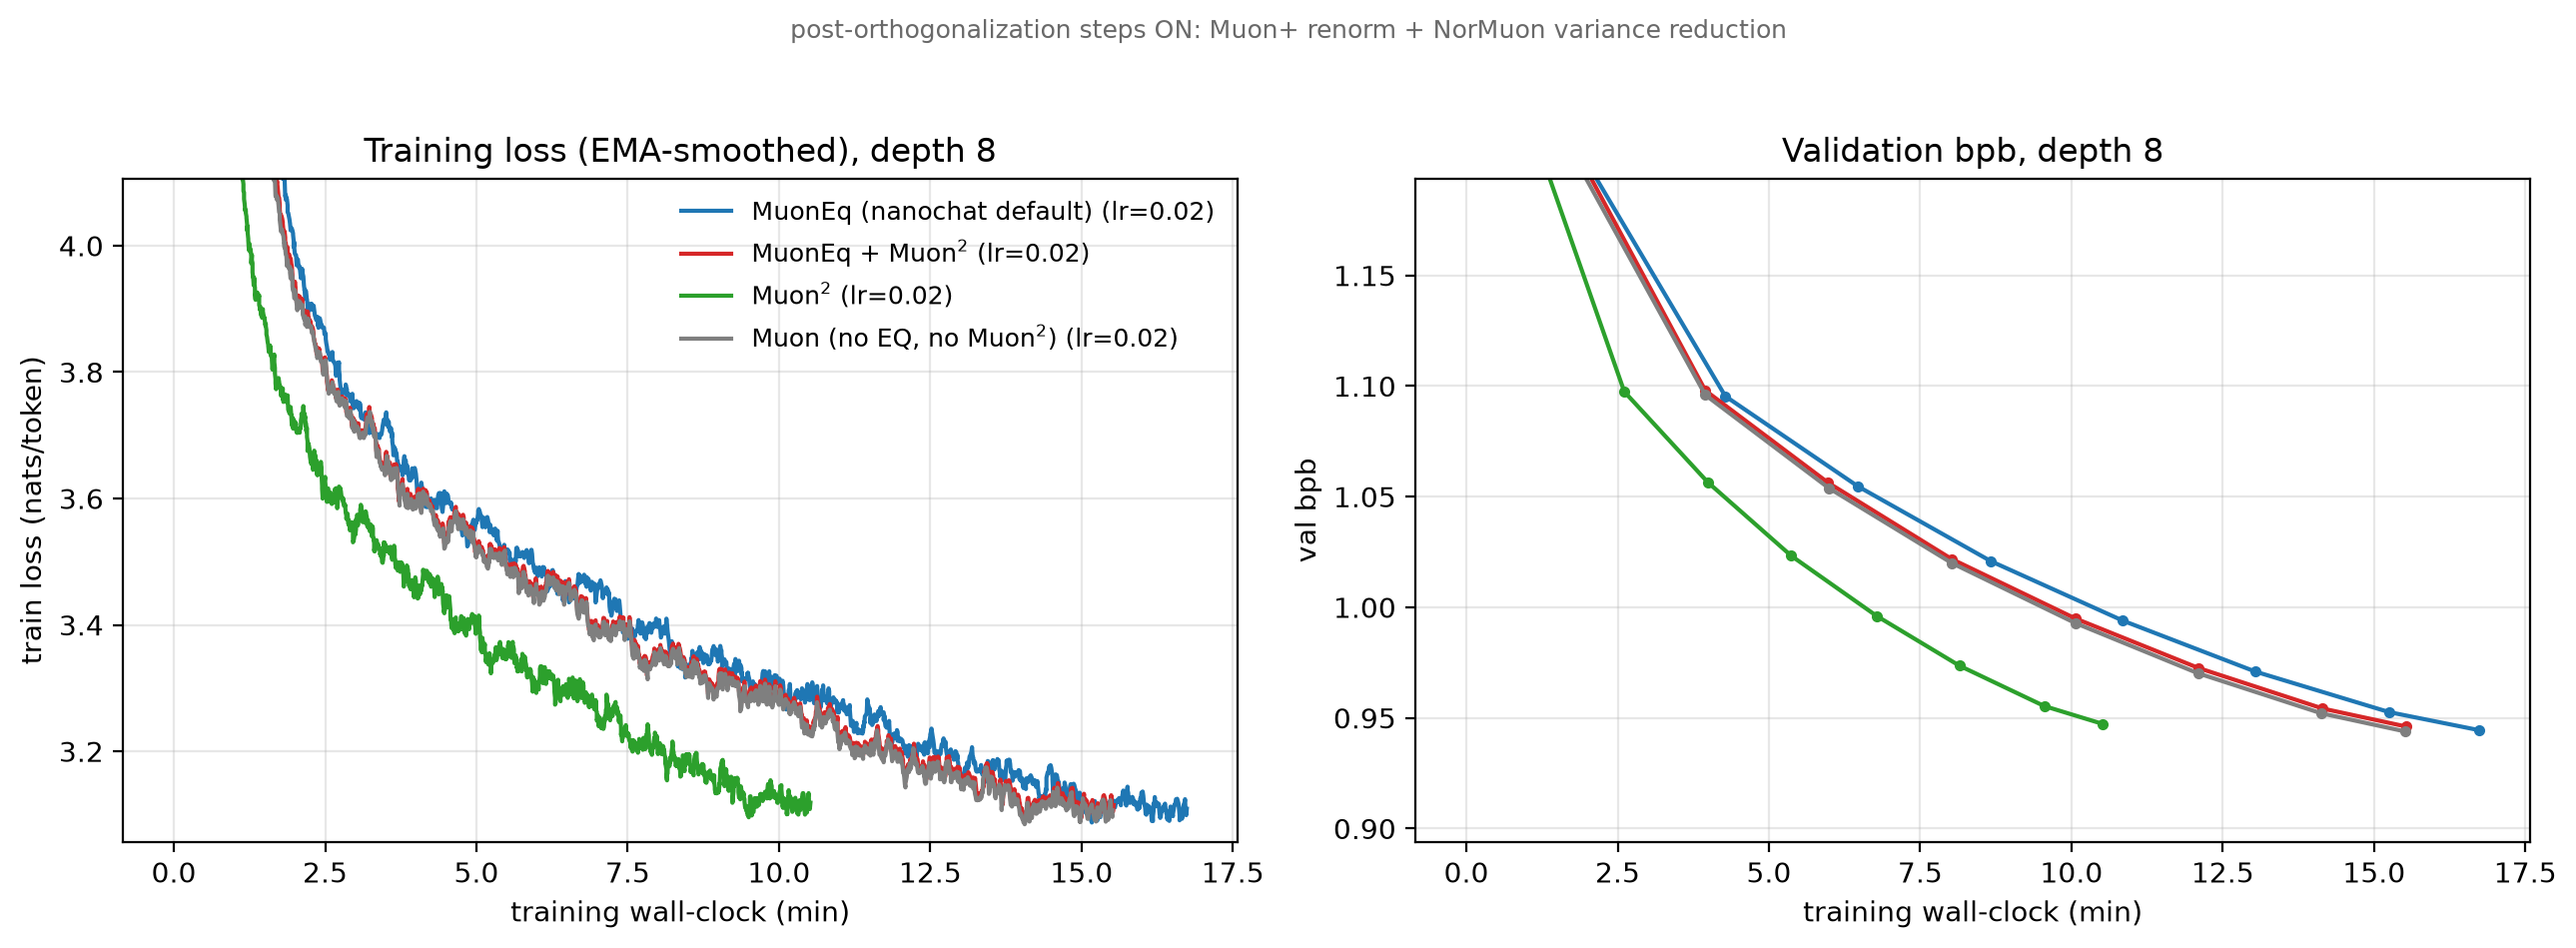
\includegraphics[width=\linewidth]{results/figures/sweep_postorth_d8_loss_val_vs_wallclock.png}
    \caption{Results at depth 8. Right: validation bpb versus wall-clock time. Left: training loss versus wall-clock time. Each curve corresponds to one optimizer variant.}
    \label{fig:postorth_d8_loss_val_vs_wallclock}
\end{figure}

\begin{figure}[t]
    \centering
    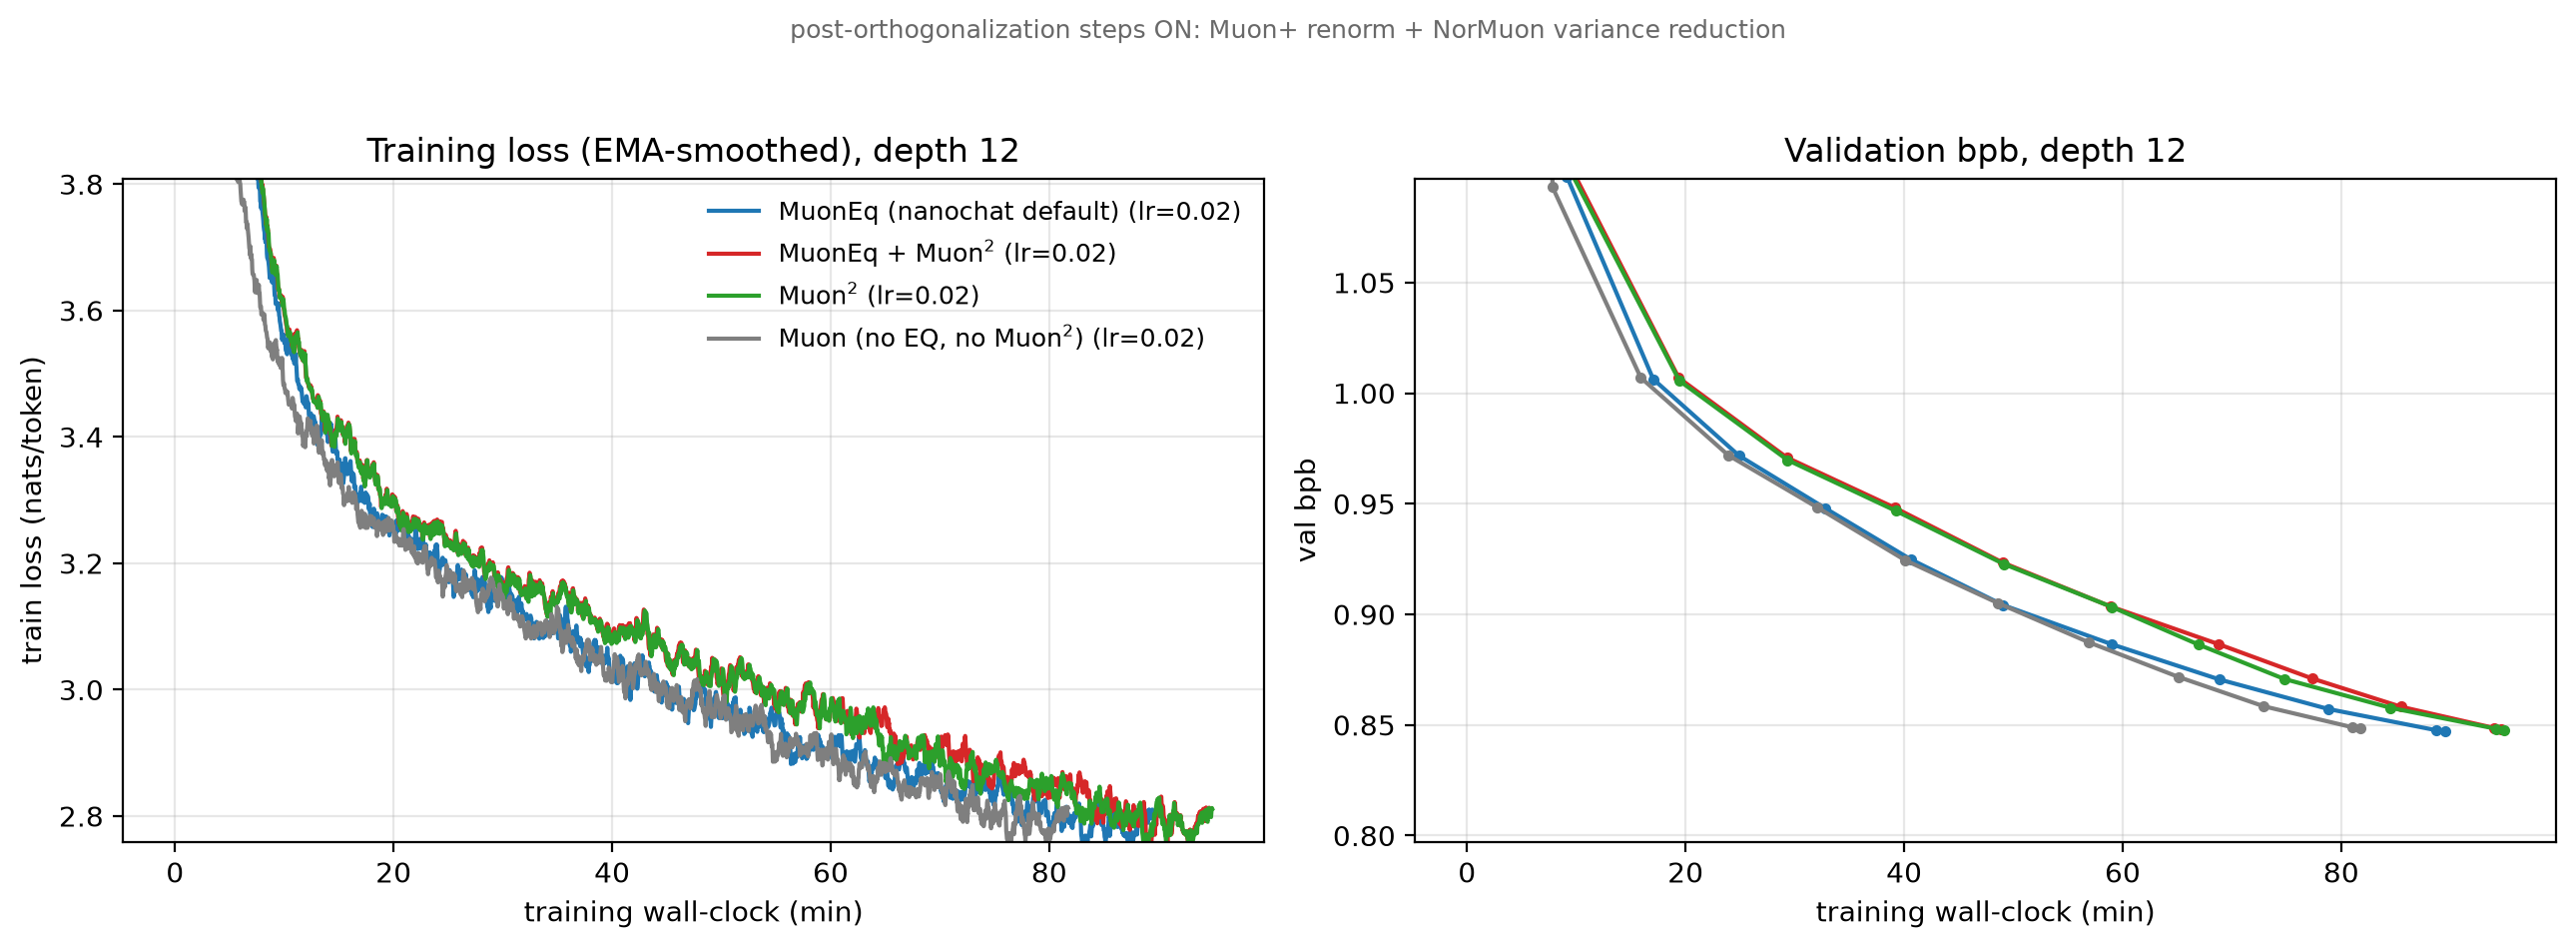
\includegraphics[width=\linewidth]{results/figures/sweep_postorth_d12_loss_val_vs_wallclock.png}
    \caption{Results at depth 12. Right: validation bpb versus wall-clock time. Left: training loss versus wall-clock time. Each curve corresponds to one optimizer variant.}
    \label{fig:postorth_d12_loss_val_vs_wallclock}
\end{figure}

\begin{figure}[t]
    \centering
    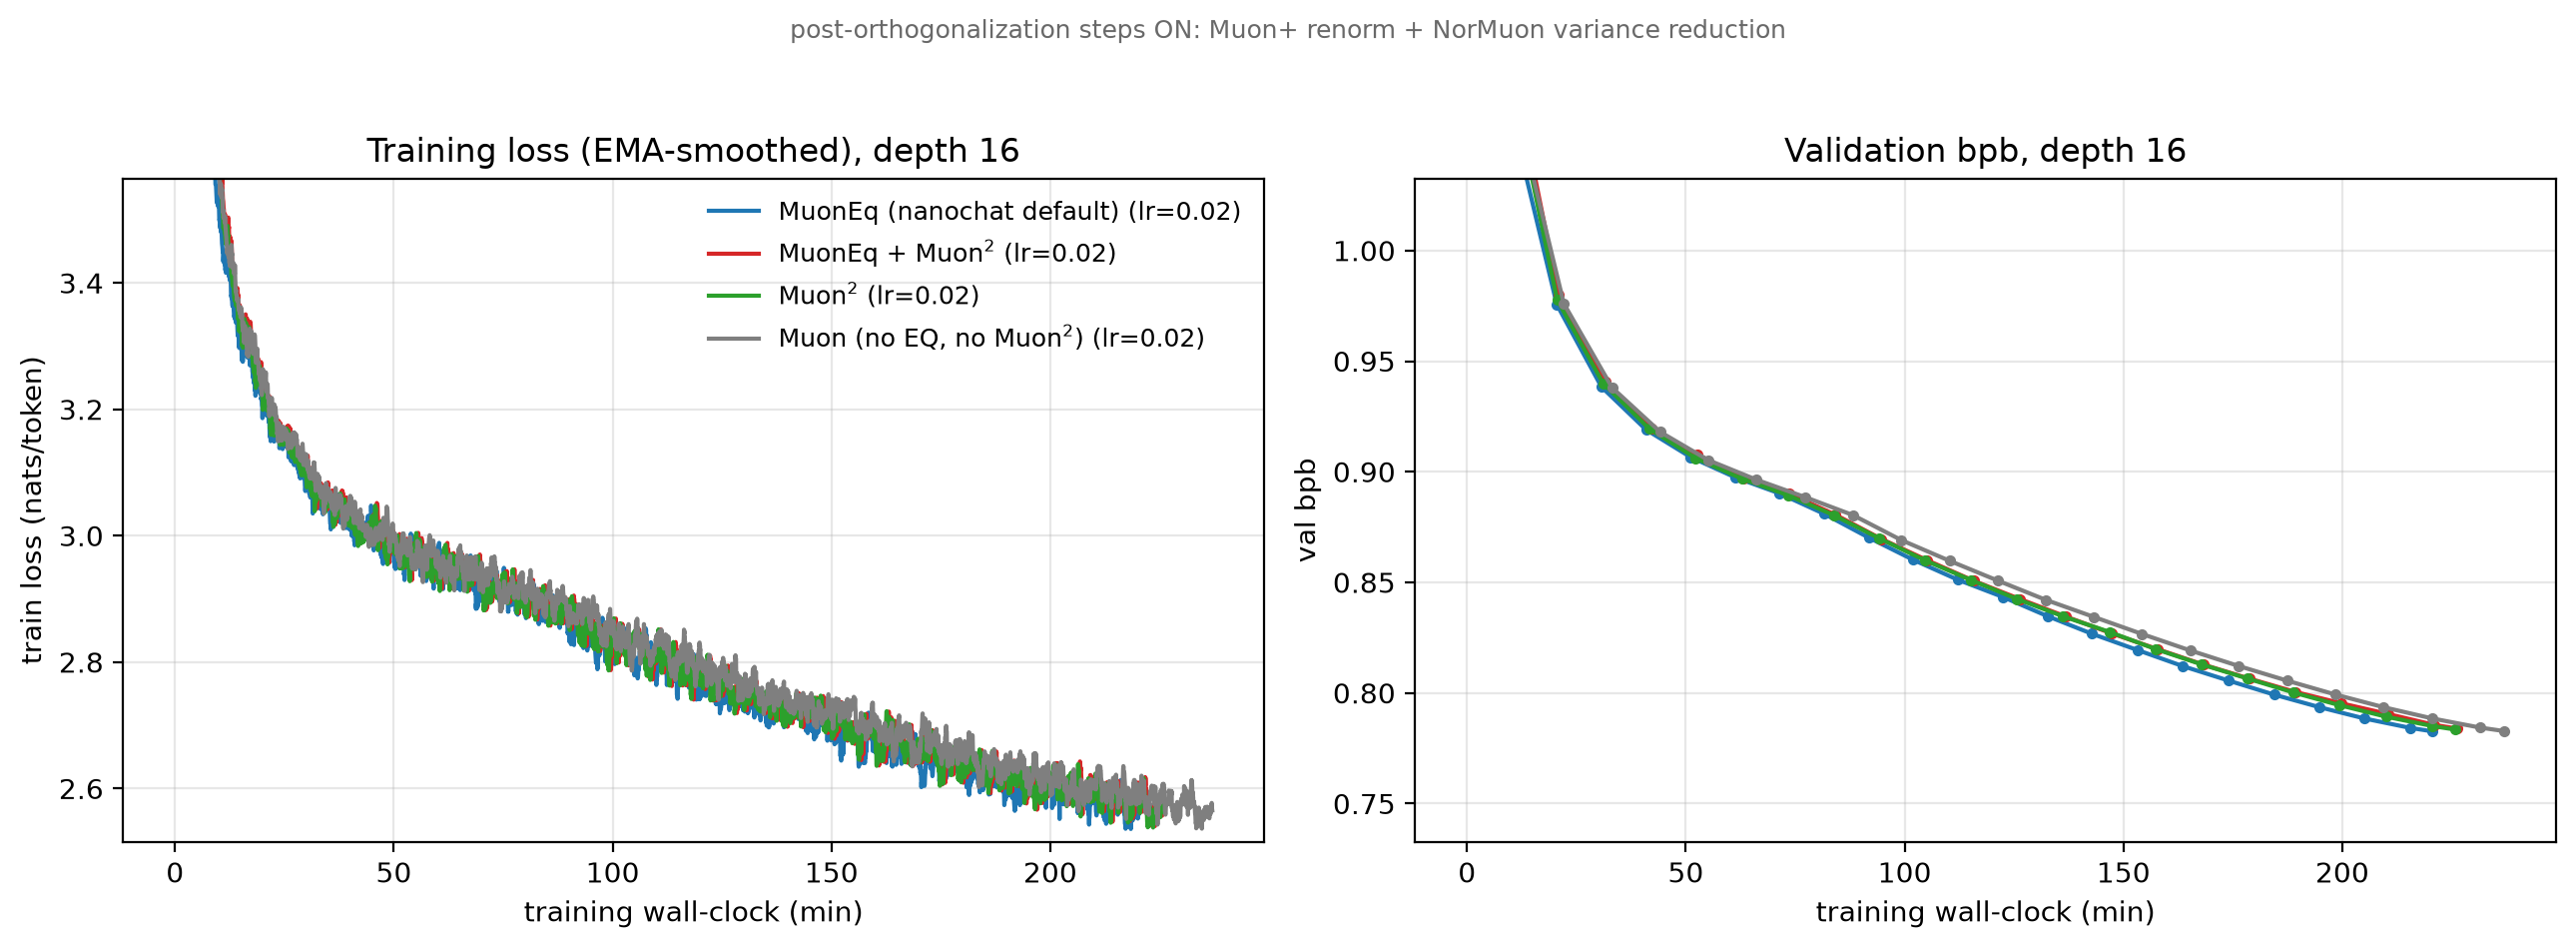
\includegraphics[width=\linewidth]{results/figures/sweep_postorth_d16_loss_val_vs_wallclock.png}
    \caption{Results at depth 16. Right: validation bpb versus wall-clock time. Left: training loss versus wall-clock time. Each curve corresponds to one optimizer variant.}
    \label{fig:postorth_d16_loss_val_vs_wallclock}
\end{figure}

\begin{figure}[t]
    \centering
    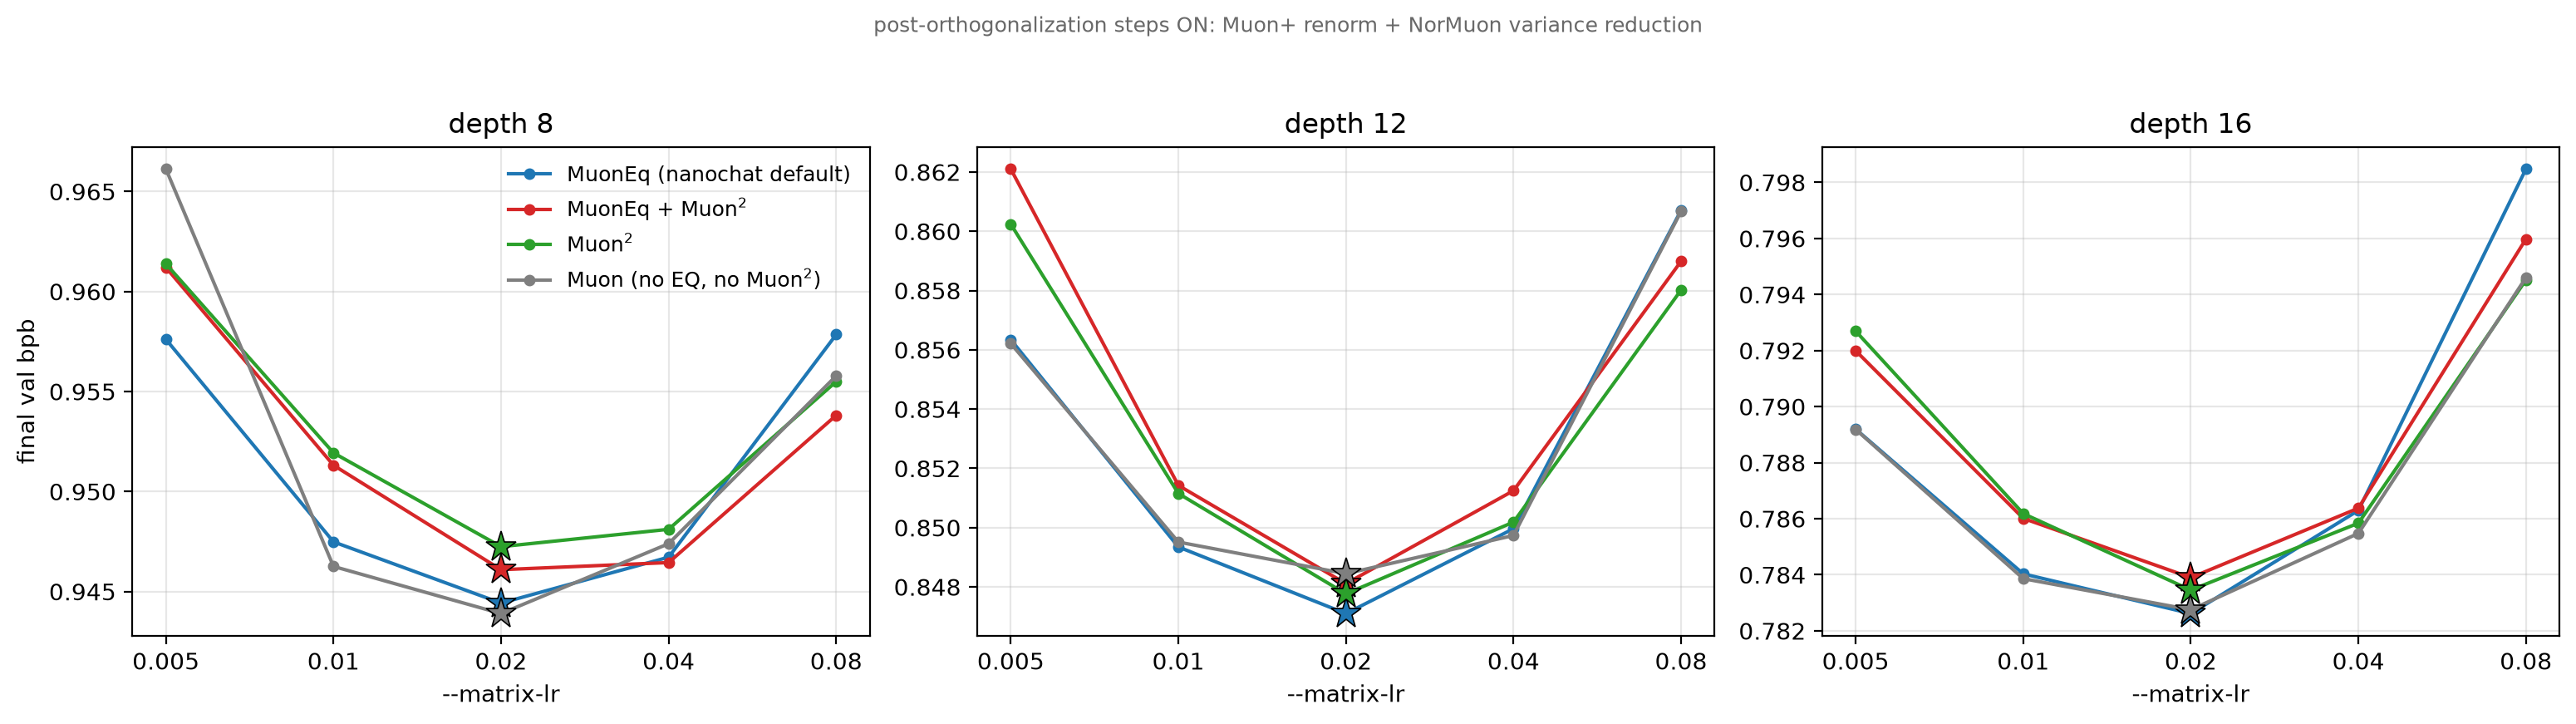
\includegraphics[width=\linewidth]{results/figures/sweep_postorth_val_bpb_vs_lr.png}
    \caption{Final validation bpb as a function of learning rate for each optimizer variant. Each subfigure corresponds to a different depth.}
    \label{fig:postorth_lr_sweep}
\end{figure}






\begin{table*}[t]
    \centering
    \footnotesize
    \setlength{\tabcolsep}{4pt}
    \caption{Training steps and wall-clock time to reach a target validation bpb. The target is the highest final validation bpb of one optimizer variant at each depth. $\Delta$ is the change relative to Base (positive = faster). Eq = MuonEq, M$^2$ = Muon$^2$.}
    \label{tab:time-to-target}
    \begin{tabular}{cclcrrrr}
        \toprule
        Depth & Target & Variant & LR & Steps & Min & $\Delta$ steps (\%) & $\Delta$ time (\%) \\
        \midrule
        8  & 0.9472 & Base      & 0.02 & 1850 & 14.94  &  0.0 &   0.0 \\
           &        & +Eq       & 0.02 & 1861 & 16.23  & -0.6 &  -7.9 \\
           &        & +Eq+M$^2$ & 0.02 & 1896 & 15.33  & -2.4 &  -2.5 \\
           &        & +M$^2$    & 0.02 & 1920 & 10.52  & -3.6 &  42.1 \\
        \midrule
        12 & 0.8484 & Base      & 0.02 & 2520 & 81.73  &  0.0 &   0.0 \\
           &        & +Eq       & 0.02 & 2478 & 87.85  &  1.7 &  -7.0 \\
           &        & +Eq+M$^2$ & 0.02 & 2507 & 94.23  &  0.5 & -13.3 \\
           &        & +M$^2$    & 0.02 & 2495 & 93.99  &  1.0 & -13.0 \\
        \midrule
        16 & 0.7839 & Base      & 0.02 & 5284 & 233.00 &  0.0 &   0.0 \\
           &        & +Eq       & 0.02 & 5275 & 216.49 &  0.2 &   7.6 \\
           &        & +Eq+M$^2$ & 0.02 & 5376 & 226.18 & -1.7 &   3.0 \\
           &        & +M$^2$    & 0.02 & 5341 & 224.32 & -1.1 &   3.9 \\
        \bottomrule
    \end{tabular}
\end{table*}



\paragraph{Results.}
At depth 8, Muon$^2$ is considerably faster to finish training and also reaches the target validation bpb fastest (Table~\ref{tab:time-to-target}). However, it ends with the highest final validation bpb of the four variants. MuonEq takes the longest to finish training but achieves the second to lowest validation bpb, were base has the lowest (Table~\ref{tab:results}).

At depth 12, base is the fastest to finish training and reaches the target validation bpb the fastest (Table~\ref{tab:time-to-target}). MuonEq achieves the lowest validation bpb, while base has the highest (Table~\ref{tab:results}). 

At depth 16, MuonEq achieves the lowest validation bpb and also the best time-to-target. Across all depths, the combined variant has higher validation bpb than MuonEq. 

\paragraph{Discussion.}
For final validation bpb, base Muon performs the best for depth 8 while MuonEq performs the best for depth 12 and 16. The results indicate that the combined variant with Muon$^2$ and MuonEq does not help the final validation bpb. It is higher compared to just using MuonEq for all depths. 

In terms of speed, however, there is no clear pattern. Time-to-target rankings differ between depths, and the percentage speed-ups relative to Base vary widely. Notably, Muon$^2$ achieves a 42.1\% speed-up over Base at depth 8, whereas the best speed-up at depth 16 is only 7.6\% (MuonEq). At depth 12, Base is even the fastest to target. 

From Table~\ref{tab:results}, we see that the median ms/step is inconsistent with what we expect from the optimizers. While it has been observed that Muon$^2$ can achieve better or similar validation loss given fewer NS-iterations, it is not applicable in our case as we used a constant 5 Polar express iterations for each variant \cite{liu-etal-2026-muon2}. In order for Muon$^2$ to obtain similar progress on loss for less compute, it needs to lower the number of NS/polar express iterations. Furthermore, MuonEq has been shown to have a slight overhead compared to standard Muon \cite{chang2026muoneqbalancingorthogonalizationlightweight}. All in all, we expect the median time per step for every optimizer with extensions (i.e. Muon$^2$ and MuonEq) to be greater than that of base. This does not happen, in fact Muon$^2$ is significantly faster at depth 8 with 328 ms/step compared to Base with 488 ms/step (Table~\ref{tab:results}). One can find more such cases across depths. In conclusion, this indicates that the median time per step is not representative of how the optimizer variants perform in regards to time.

A wise choice would have been to investigate this immediately, by running multiple runs with the exact same setup. However, this was not noted at the time of finishing experiment set 1. Instead, further investigation of the optimizers themselves was conducted, as will be shown in experiment set 2. Section~\ref{Time-error-analysis} covers the experiments investigating the time errors. 


\subsection{Pre-Training GPT without post-orthogonalization}
\label{sec:Pre-Training-GPT-without-post-orthogonalization}

Since the results of the first set of experiments showed no clear pattern across depths in terms of time, we ran an additional set of experiments with simplified optimizers. In particular, we removed both post-orthogonalization extensions, so the base variant in these experiments is plain Muon with Polar Express iterations and Nesterov-style momentum. We again evaluate four variants: Base, MuonEq, Muon$^2$, and MuonEq + Muon$^2$.

For the hyperparameters that were held constant, we use the same as in the first set of experiments (Table~\ref{tab:constant-hparams}). The learning rate sweep covers a smaller range centered at $0.02$, since this was the best learning rate for all optimizers in the previous sweep (Figure~\ref{fig:plain-lr-sweep}). Due to limited compute, we train only at depths 8 and 12, both on a single H100-47GB GPU.


\begin{table}[t]
    \centering
    \footnotesize
    \setlength{\tabcolsep}{3.5pt}
    \caption{Final validation bpb, training loss, and speed per variant and depth for the baseline without post-orthogonalization extensions. ms/step is the median time for each step. The learning rate for each run was chosen by lowest val bpb from the sweep. Eq = MuonEq, M$^2$ = Muon$^2$.}
    \label{tab:plain-results}
    \pgfplotstabletypeset[
        col sep=comma,
        columns={depth, variant, lr, final_val_bpb, final_train_loss, train_min, median_ms_per_step},
        every head row/.style={before row=\toprule, after row=\midrule},
        every last row/.style={after row=\bottomrule},
        every row no 4/.style={before row=\midrule},
        columns/depth/.style={column name=Depth, int detect, column type=c},
        columns/variant/.style={
            column name=Variant, string type, column type=l,
            % eq_m2 must come before eq and m2
            string replace*={eq_m2}{+Eq+M$^2$},
            string replace*={eq}{+Eq},
            string replace*={m2}{+M$^2$},
            string replace*={base}{Base},
        },
        columns/lr/.style={column name=LR, fixed, precision=2, zerofill, column type=c},
        columns/final_val_bpb/.style={column name=Val bpb, fixed, precision=4, zerofill, column type=c},
        columns/final_train_loss/.style={column name=Loss, fixed, precision=3, zerofill, column type=c},
        columns/train_min/.style={column name=Min, fixed, precision=1, zerofill, column type=c},
        columns/median_ms_per_step/.style={column name=ms/step, fixed, precision=0, column type=c},
    ]{results/tables/plain_selected_runs.csv}
\end{table}


\begin{figure}[t]
    \centering
    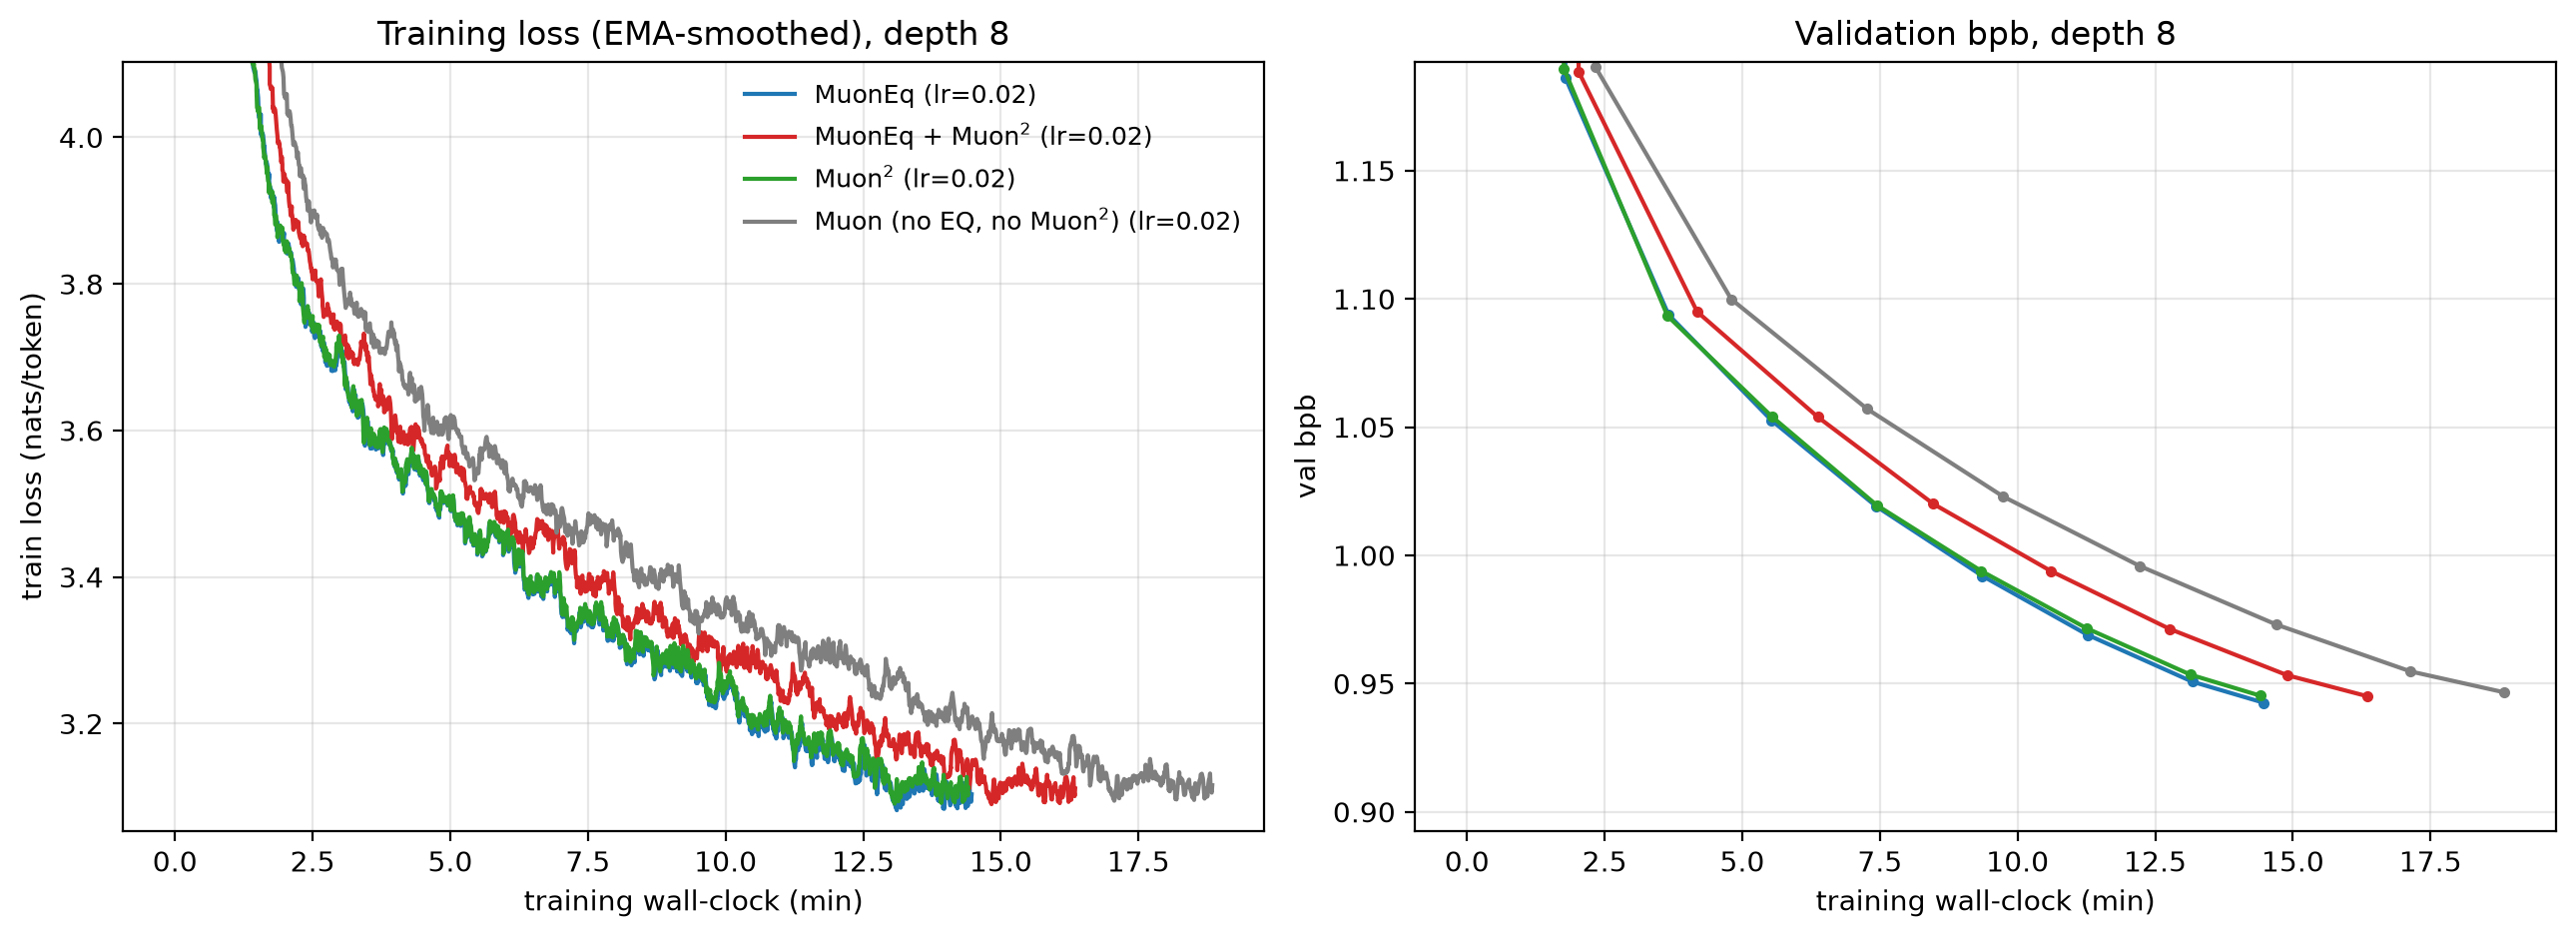
\includegraphics[width=\linewidth]{results/figures/plain_d8_loss_val_vs_wallclock.png}
    \caption{Depth 8: Training loss (left) and validation bpb (right) versus wall-clock time at depth 8 for the baseline without post-orthogonalization extensions, for each variant.}
    \label{fig:plain-d8-wallclock}
\end{figure}

\begin{figure}[t]
    \centering
    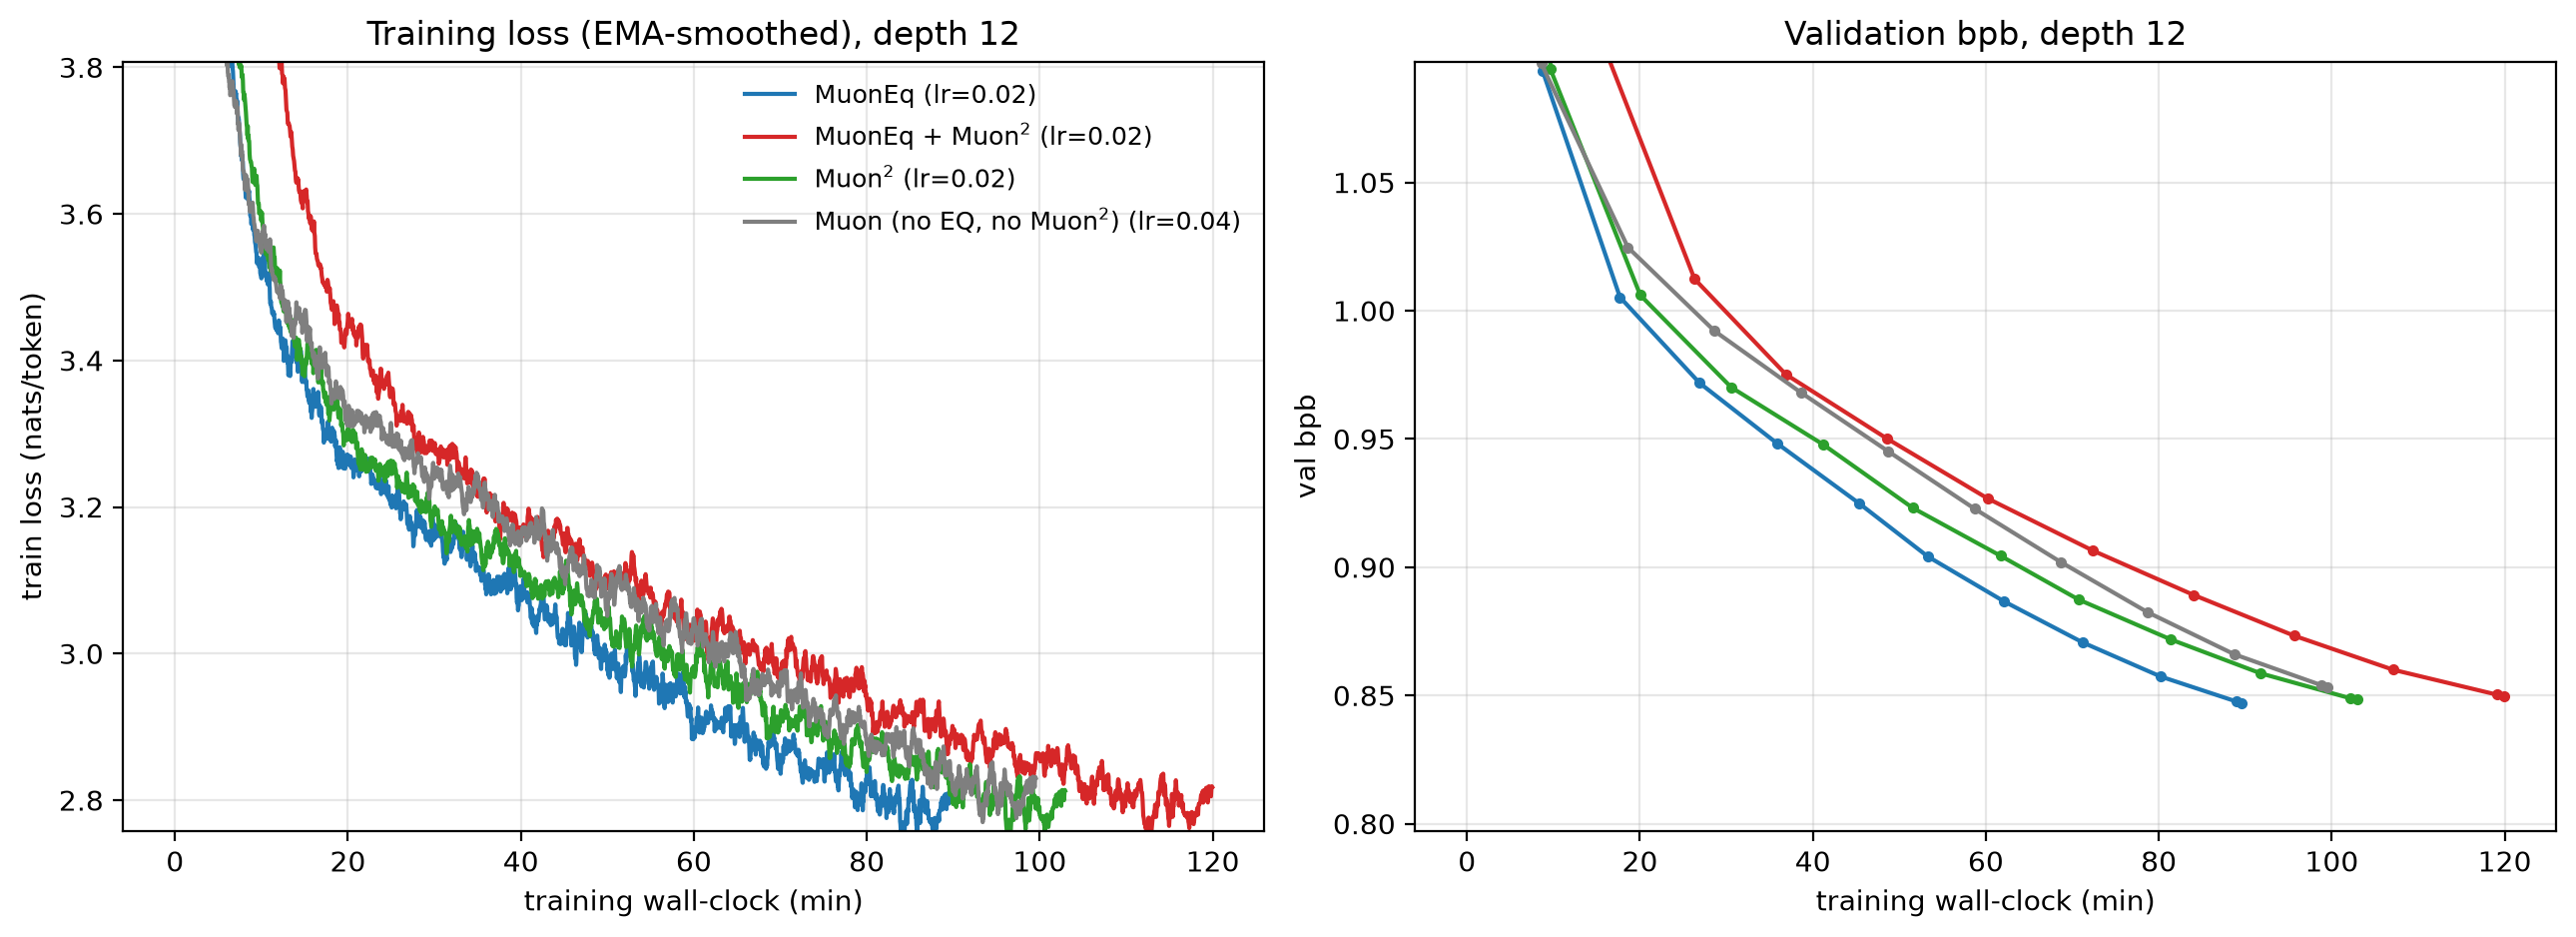
\includegraphics[width=\linewidth]{results/figures/plain_d12_loss_val_vs_wallclock.png}
    \caption{Depth 12: Training loss (left) and validation bpb (right) versus wall-clock time at depth 12 for the baseline without post-orthogonalization extensions, for each variant.}
    \label{fig:plain-d12-wallclock}
\end{figure}


\begin{figure}[t]
    \centering
    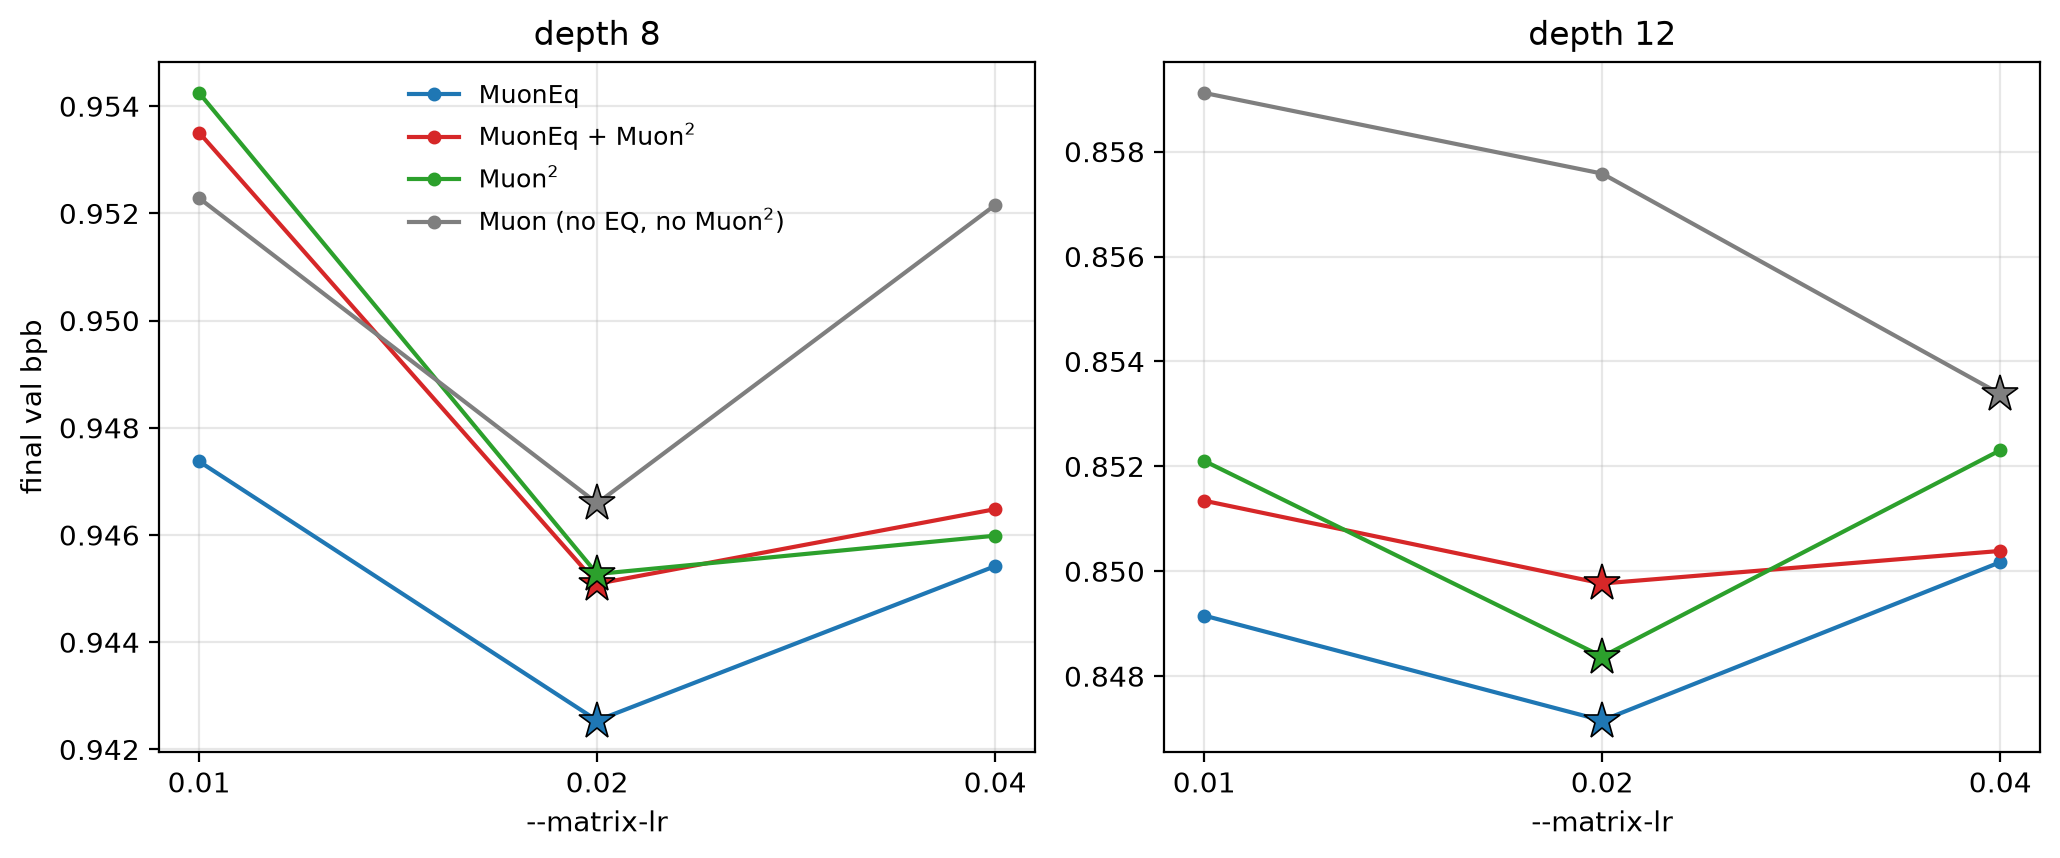
\includegraphics[width=\linewidth]{results/figures/plain_val_bpb_vs_lr.png}
    \caption{Final validation bpb as a function of learning rate for each optimizer variant without post-orthogonalization extensions. Each subfigure corresponds to a different depth.}
    \label{fig:plain-lr-sweep}
\end{figure}



\begin{table*}[t]
    \centering
    \footnotesize
    \setlength{\tabcolsep}{4pt}
    \caption{Training steps and wall-clock time to reach a target validation bpb for the baseline without post-orthogonalization extensions. The target is the final validation bpb of Base. $\Delta$ is the speedup relative to Base (positive = faster). Eq = MuonEq, M$^2$ = Muon$^2$.}
    \label{tab:plain-time-to-target}
    \pgfplotstabletypeset[
        col sep=comma,
        columns={depth, target, variant, lr, steps_to_target, minutes_to_target, speedup_steps_pct, speedup_time_pct},
        % keep only the val bpb rows (rows 0-3 and 8-11 of the CSV)
        row predicate/.code={%
            \pgfmathparse{int(mod(#1,8)>3)}%
            \ifnum\pgfmathresult=1 \pgfplotstableuserowfalse\fi
        },
        every head row/.style={before row=\toprule, after row=\midrule},
        every last row/.style={after row=\bottomrule},
        every row no 4/.style={before row=\midrule},
        every row no 8/.style={before row=\midrule},
        columns/depth/.style={column name=Depth, int detect, column type=c},
        columns/target/.style={column name=Target, fixed, precision=4, zerofill, column type=c},
        columns/variant/.style={
            column name=Variant, string type, column type=l,
            % eq_m2 must come before eq and m2
            string replace*={eq_m2}{+Eq+M$^2$},
            string replace*={eq}{+Eq},
            string replace*={m2}{+M$^2$},
            string replace*={base}{Base},
        },
        columns/lr/.style={column name=LR, fixed, precision=2, zerofill, column type=c},
        columns/steps_to_target/.style={column name=Steps, fixed, precision=0, column type=r},
        columns/minutes_to_target/.style={column name=Min, fixed, precision=1, zerofill, column type=r},
        columns/speedup_steps_pct/.style={column name=$\Delta$ steps (\%), fixed, precision=1, zerofill, column type=r},
        columns/speedup_time_pct/.style={column name=$\Delta$ time (\%), fixed, precision=1, zerofill, column type=r},
    ]{results/tables/plain_time_to_target.csv}
\end{table*}




\paragraph{Results.}
We first note that the learning rate sweep is problematic for the Base variant at depth 12. Its best learning rate lies at the edge of the sweep (0.04), so a larger learning rate may well be better (Table~\ref{tab:plain-val-bpb-vs-lr}, Figure~\ref{fig:plain-lr-sweep}). We therefore draw conclusions about Base, relative to the other variants, with more caution.

MuonEq achieves the lowest final validation bpb at both depths (Table~\ref{tab:plain-results}). It is also the fastest to reach the target at both depths (Table~\ref{tab:plain-time-to-target}). Base has the highest validation bpb for both depths.

The combined Muon$^2$ and MuonEq variant underperforms relative to using either extension individually. At depth 8 it is still faster to the target than Base, but at depth 12 it is slower. Its final validation bpb is nevertheless lower than that of Base at both depths, and higher than that of either extension alone.

\paragraph{Discussion.}

MuonEq performs best in both validation bpb and time-to-target. However, the time-to-target results are unreliable because of the issues discussed in Section~\ref{sec:Pre-Training-GPT-without-post-orthogonalization} and analysed in Section~\ref{Time-error-analysis}. The only result indicating a benefit of the combined variant over any individual variant is the final validation bpb at depth 8, where it is lower than that of Muon$^2$ alone. Overall, these results again suggest that the combined variant is worse than using the MuonEq extension on its own. Furthermore, the results are inconclusive as to whether the combined variant is better than Muon$^2$ alone.

The same issue with the median ms/step is present in this set of experiments. We observe behavior similar to that noted in the discussion of Section~\ref{Pre-Training GPT with post-orthogonalization}, where the base variant has a slower median ms/step than the other variants.


\subsection{Comparing results between the experiments}
\label{Comparing-results-between-the-experiments}

We now perform a few comparisons between the experiment sets, to investigate whether the post-orthogonalisation extensions benefit the optimizer variants. We note that comparisons are made only between depths 8 and 12, as we did not run depth 16 for post-orthogonalization turned off.


\begin{figure*}[t]
    \centering
    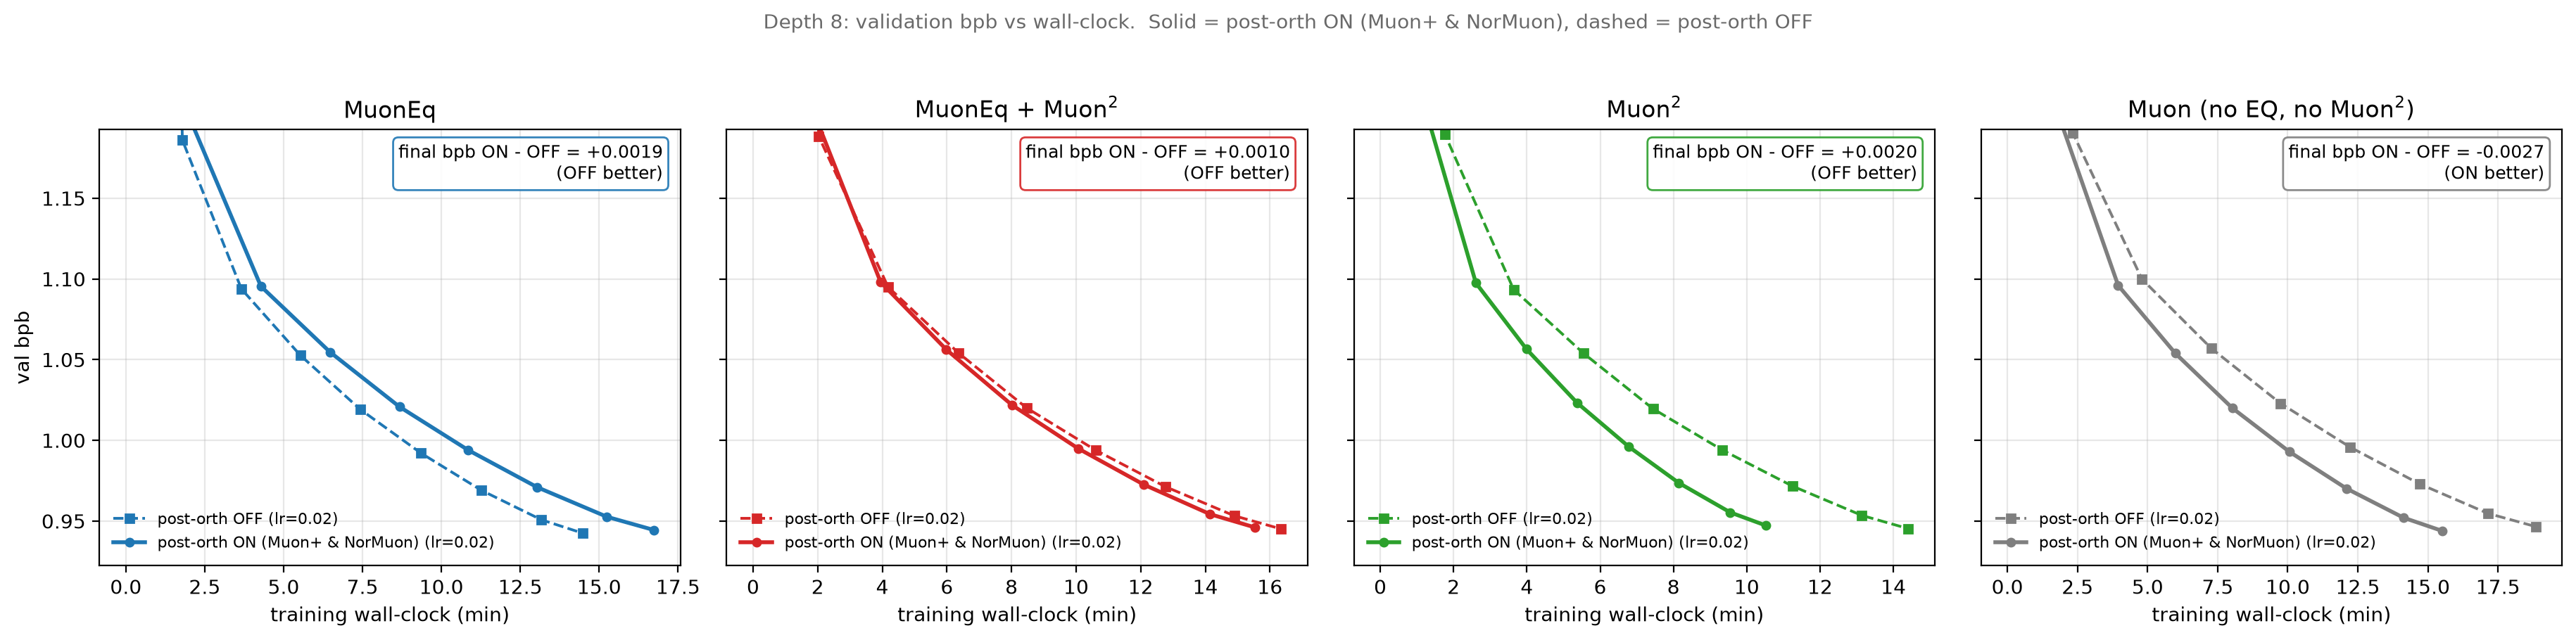
\includegraphics[width=\textwidth]{results/figures/compare_postorth_d8_val_bpb_vs_wallclock.png}
    \caption{Depth 8: Validation bpb versus wall-clock time, comparing the post-orthogonalization extensions (Muon+ and NorMuon) for each optimizer variant. ON/OFF better only looks at the final bpb. If it is lower, it is considered better. }
    \label{fig:compare-postortho-d8}
\end{figure*}

\begin{figure*}[t]
    \centering
    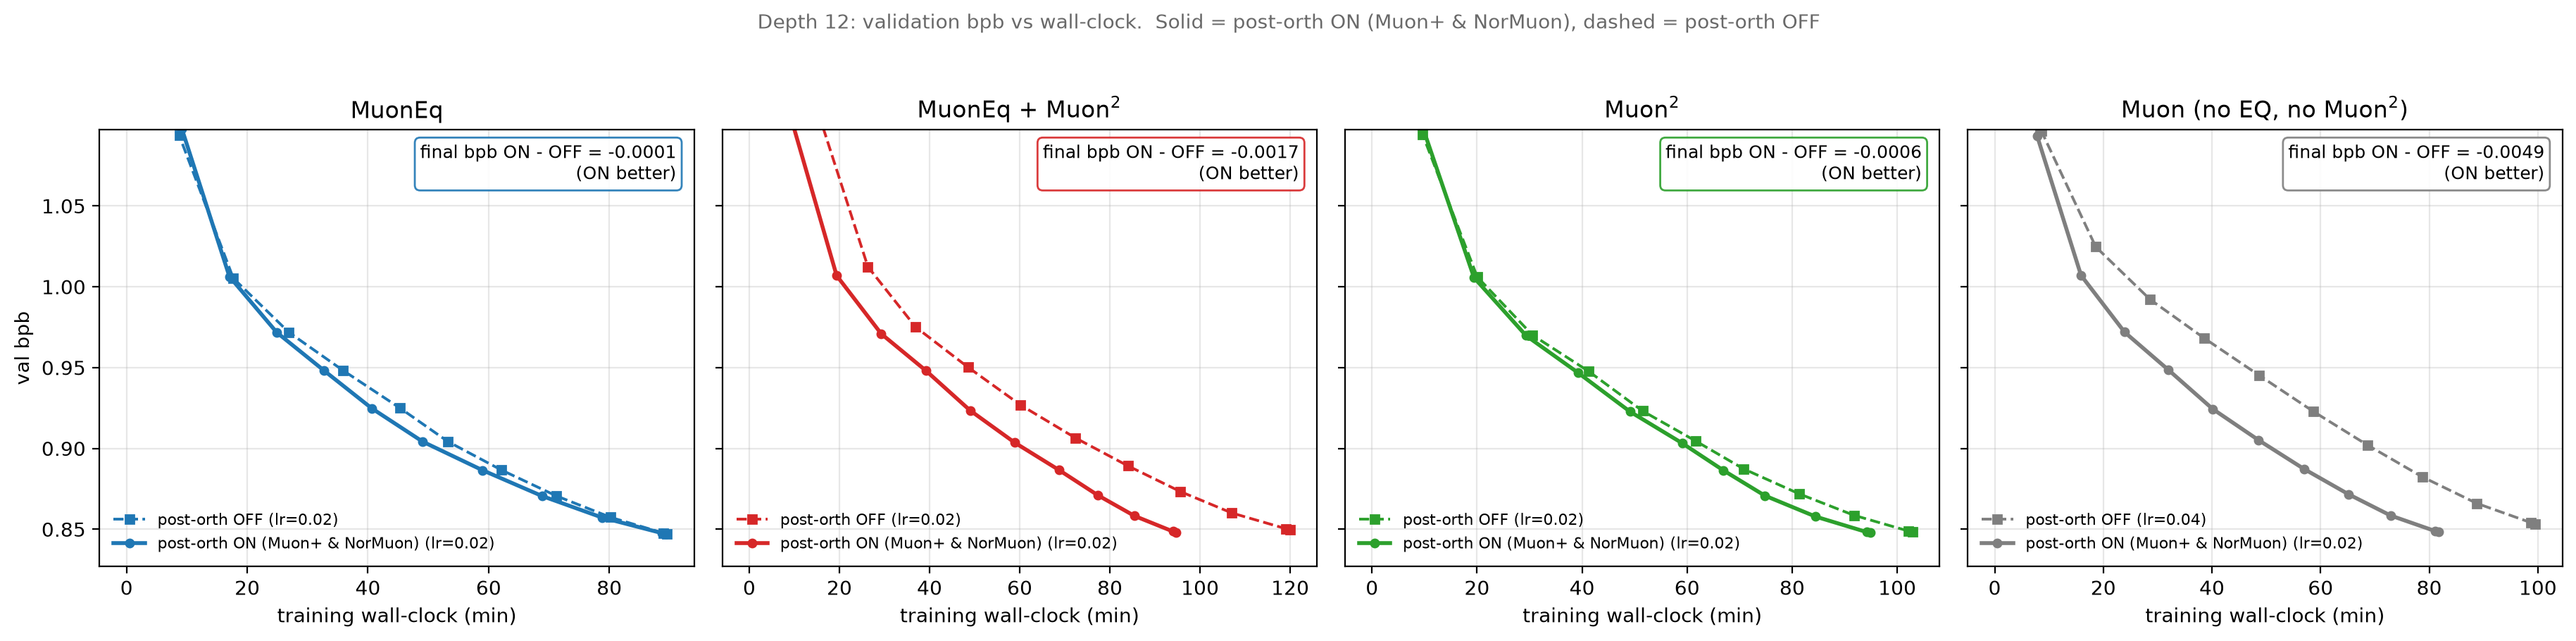
\includegraphics[width=\textwidth]{results/figures/compare_postorth_d12_val_bpb_vs_wallclock.png}
    \caption{Depth 12: Validation bpb versus wall-clock time, comparing the post-orthogonalization extensions (Muon+ and NorMuon) for each optimizer variant. ON/OFF better only looks at the final bpb. If it is lower, it is considered better. }
    \label{fig:compare-postortho-d12}
\end{figure*}



\begin{table*}[t]
\centering
\small
\begin{tabular}{llccc}
\toprule
 & & \multicolumn{2}{c}{Final val.\ bpb} & \\
\cmidrule(lr){3-4}
Depth & Variant & Post-orth.\ ON & Post-orth.\ OFF & $\Delta$ (ON $-$ OFF) \\
\midrule
\multirow{4}{*}{8}
 & Base        & \textbf{0.9439} & 0.9466 & $-0.0027$ \\
 & +Eq         & 0.9444 & \textbf{0.9425} & $+0.0019$ \\
 & +Eq+M$^2$   & 0.9461 & 0.9451 & $+0.0010$ \\
 & +M$^2$      & 0.9472 & 0.9453 & $+0.0020$ \\
\midrule
\multirow{4}{*}{12}
 & Base        & 0.8484 & 0.8534$^{\dagger}$ & $-0.0049$ \\
 & +Eq         & \textbf{0.8471} & \textbf{0.8472} & $-0.0001$ \\
 & +Eq+M$^2$   & 0.8481 & 0.8498 & $-0.0017$ \\
 & +M$^2$      & 0.8478 & 0.8484 & $-0.0006$ \\
\bottomrule
\end{tabular}
\caption{Final validation bpb with post-orthogonalization extensions (Muon+ and NorMuon) ON (first set of experiments) and OFF (second set). Eq = MuonEq, M$^2$ = Muon$^2$. $\Delta < 0$ means ON is better. Bold marks the best variant per depth and column. All runs use matrix LR $0.02$ except $^{\dagger}$, where the best LR was $0.04$, at the edge of the sweep.}
\label{tab:on-vs-off}
\end{table*}


The results are mixed: for some variants, enabling the post-orthogonalization extensions improves validation bpb, while for others it does not (Table~\ref{tab:on-vs-off}). In particular, the effect does not generalize across the two depths. For MuonEq, Combined, and Muon$^2$, having the extensions OFF is better at depth 8, whereas having them ON is better at depth 12.

For the base variant, however, turning the setting ON improves validation bpb, and this variant also shows the largest difference in validation bpb between the two settings. Since we cannot analyze the timing properly, we cannot judge whether this translates into faster training convergence.

Looking at MuonEq alone, at depth 8 it reaches the lowest final validation bpb of all variants, ON and OFF, with the lowest when extensions is OFF. As this setting is better when OFF, the results suggest that MuonEq performs better without post-orthogonalization. Since Muon+ and NorMuon necessarily add compute, it lengthens training time without improving final validation bpb, hence it cannot perform better ON given the result at depth 8. However, this does not generalize across depths, as MuonEq is better with the extensions ON at depth 12. The difference there is significantly smaller, only $-0.0001$ in validation bpb.


\subsection{Time error analysis}
\label{Time-error-analysis}

Finally, a third set of experiments investigated whether the unexpected timing results were caused by differences between the physical GPUs on the cluster. For this purpose, we performed eight identical runs on a single H100 47 GB GPU. All hyperparameters held constant in the earlier experiments retained their previous values (Table~\ref{tab:constant-hparams}). The matrix learning rate was set to 0.025, and we used the MuonEq variant with post-orthogonalization enabled.

\begin{figure*}[t]
    \centering
    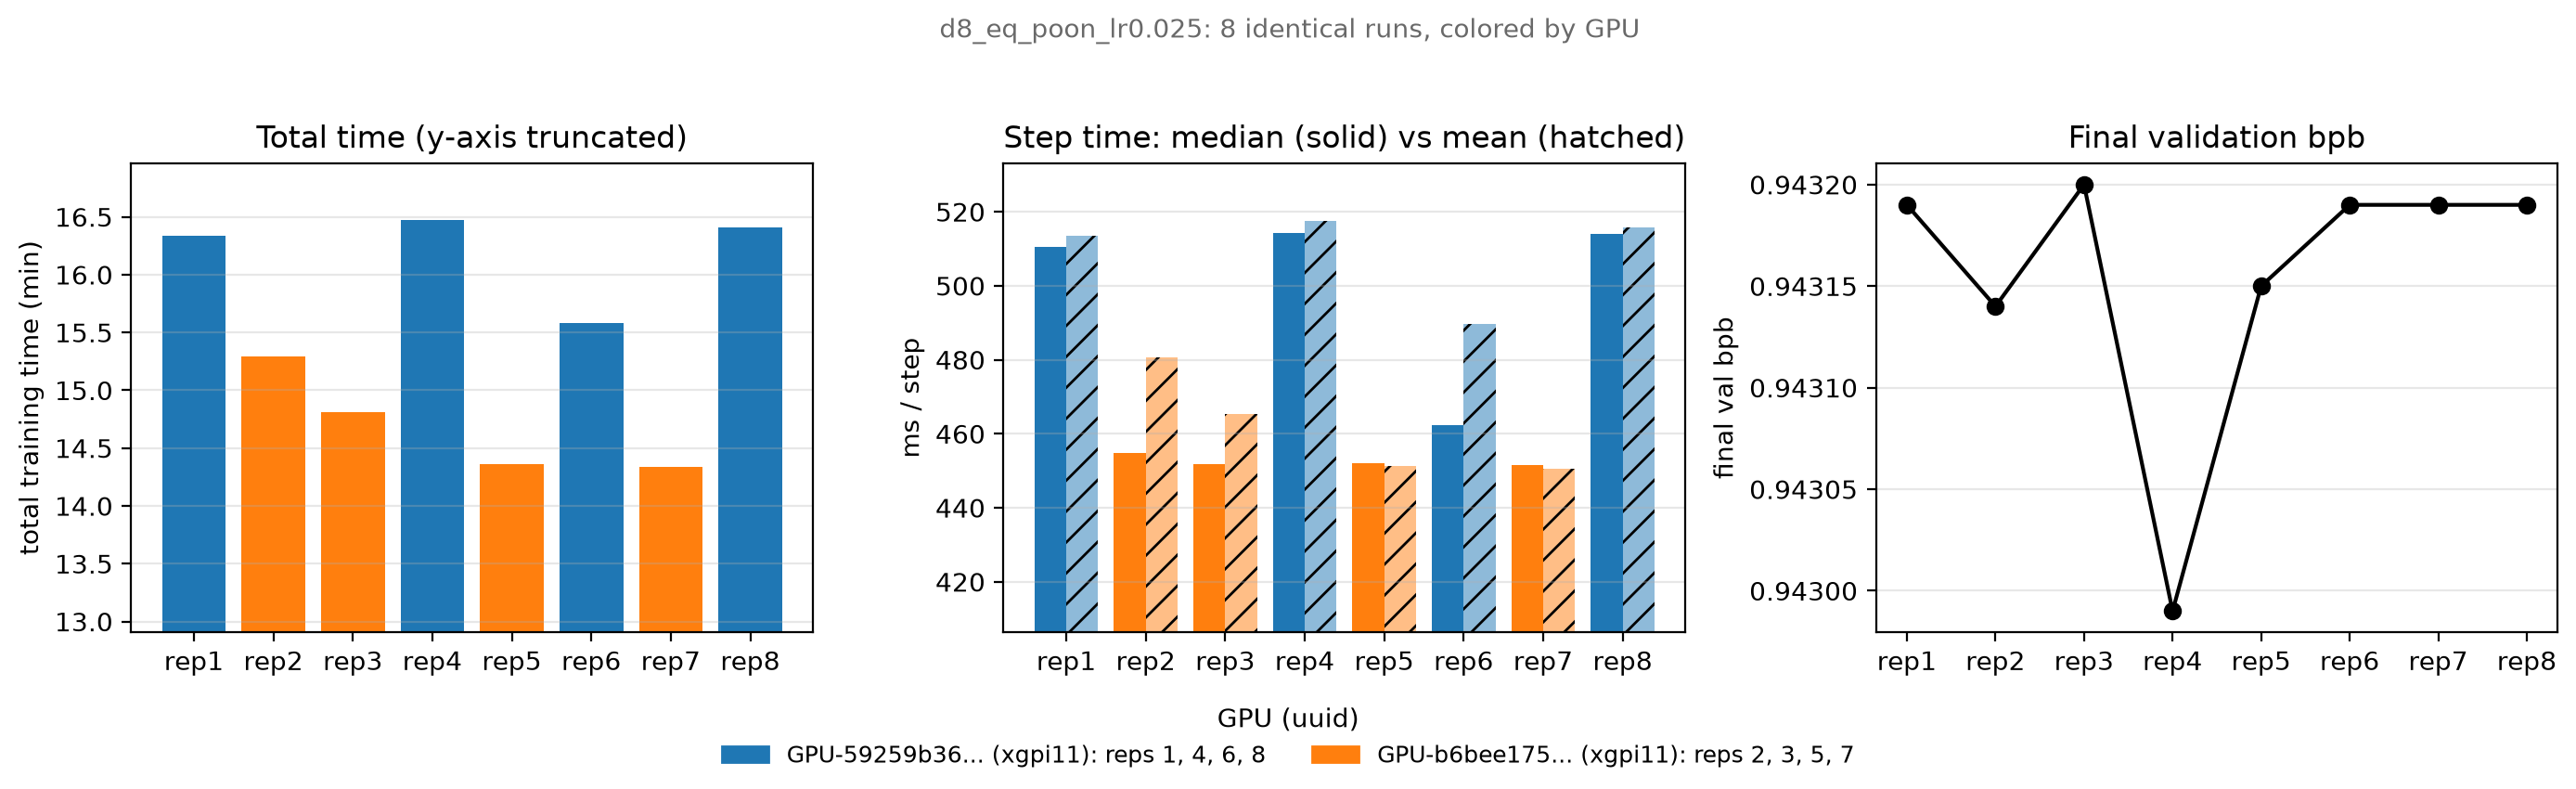
\includegraphics[width=\textwidth]{results/figures/timing_repeat_d8_eq_poon_lr0.025_per_run.png}
    \caption{Run-to-run variability of eight identical runs (depth 8, MuonEq, learning rate $0.025$), colored by the exact physical GPU they ran on. Left: total training time (y-axis truncated). Middle: median and mean time per step. Right: final validation bpb.}
    \label{fig:med-time-gpus}
\end{figure*}


Figure~\ref{fig:med-time-gpus} shows that the two GPUs, although located on the same node, yield clearly different timings. Runs on GPU~1 (blue; runs 1, 4, 6, 8) are generally slower than those on GPU~2 (orange; runs 2, 3, 5, 7), with total training times ranging from about 14.3 to 16.5 minutes. In contrast, the final validation bpb varies by only about $2\times10^{-4}$ across runs.

We conclude that the unexpected timing results from experiment sets 1 and 2 are due to the use of different physical GPUs. The mechanism by which the GPUs produce different timings is not entirely clear. One possibility is that the GPUs themselves differ enough in performance to account for the gap. Another is that other jobs were running on one of the GPUs but not on the other.

Despite this contamination of the results from experiment sets 1 and 2, we maintain that our conclusions based on final validation bpb remain valid, since this metric is not affected by timing. The differences in final validation bpb across the identical runs were at most $2\times10^{-4}$, whereas the differences observed in experiment sets 1 and 2 were larger.



\section{Conclusion}
\label{Conclusion}

Results that depend on time should be disregarded. In particular, our timing error analysis shows that run times are significantly affected by which physical GPU is used, so the timing results are contaminated. 

The combined variant, which uses both MuonEq and Muon$^2$, does not reduce the final validation bpb beyond what MuonEq achieves alone. Since it also requires additional computation by construction, and hence more time per step, it is strictly worse than MuonEq alone. This conclusion is independent of the median ms/step, time-to-finish, and time-to-target results.

Overall, MuonEq was the most effective at reducing the final validation bpb. However, without a proper timing results and analysis, we cannot conclude that it is better than Muon$^2$, since compute time may play a role.



\section{Future work}
\label{sec:future-work}

Our results suggest that enabling post-orthogonalization in MuonEq may not lower validation bpb compared to leaving it off. Future work could examine this across more depths and evaluate additional variants, namely NorMuon alone and Muon+ alone, each combined with MuonEq, which may help identify a stronger optimizer. 


\section*{Limitations}

The results and conclusions of this report are subject to several limitations. First, we conduct experiments at only three depths. Even findings that generalize across these depths may not hold for model sizes larger than depth 16 or smaller than depth 8. Second, the experiments were not run in a multi-GPU setting, which would be more representative of pre-training. Any method that benefits from such a setting would therefore not be fairly represented here.

\section*{AI Declerations}

AI (Claude) was used in the process of this project. In particular, it was used to generate and debug code, assist in understanding ideas, and help in the process of writing the report. I am responsible for the work.



\clearpage
\bibliography{references}


\clearpage
\onecolumn
\section*{Appendix}




\begin{table*}[!htbp]
    \centering
    \footnotesize
    \caption{Final validation bpb as a function of learning rate (column headers) for each variant and depth.}
    \label{tab:val-bpb-vs-lr}
    \pgfplotstabletypeset[
        col sep=comma,
        string type,
        every head row/.style={before row=\toprule, after row=\midrule},
        every last row/.style={after row=\bottomrule},
        every row no 4/.style={before row=\midrule},
        every row no 8/.style={before row=\midrule},
        columns/variant/.style={
            string replace*={eq_m2}{+Eq+M$^2$},
            string replace*={eq}{+Eq},
            string replace*={m2}{+M$^2$},
            string replace*={base}{Base},
        },
    ]{results/tables/sweep_postorth_val_bpb_vs_lr.csv}
\end{table*}


\begin{table*}[!htbp]
    \centering
    \footnotesize
    \caption{Final validation bpb as a function of learning rate (column headers) for each variant and depth, without post-orthogonalization extensions.}
    \label{tab:plain-val-bpb-vs-lr}
    \pgfplotstabletypeset[
        col sep=comma,
        string type,
        every head row/.style={before row=\toprule, after row=\midrule},
        every last row/.style={after row=\bottomrule},
        every row no 4/.style={before row=\midrule},
        every row no 8/.style={before row=\midrule},
        columns/variant/.style={
            string replace*={eq_m2}{+Eq+M$^2$},
            string replace*={eq}{+Eq},
            string replace*={m2}{+M$^2$},
            string replace*={base}{Base},
        },
    ]{results/tables/plain_val_bpb_vs_lr.csv}
\end{table*}


\begin{figure}[!htbp]
    \centering
    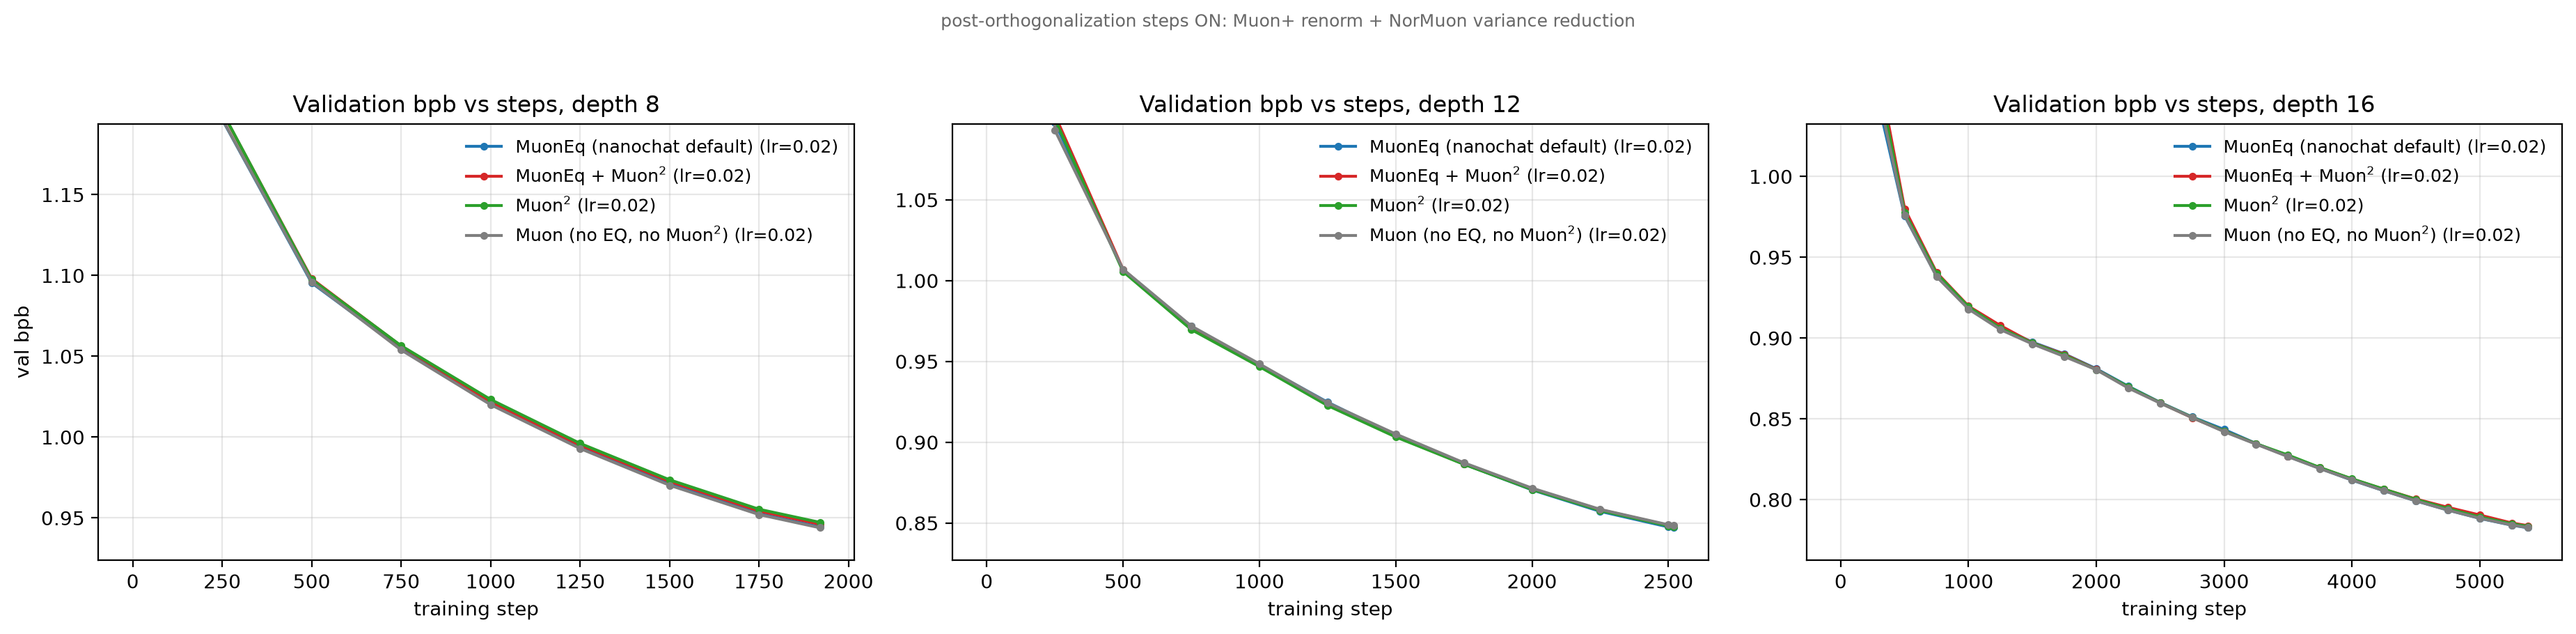
\includegraphics[width=\linewidth]{results/figures/sweep_postorth_val_bpb_vs_steps.png}
    \caption{Validation bpb as a function of training step for each optimizer variant. Each subfigure corresponds to a different depth.}
    \label{fig:postorth_val_vs_steps}
\end{figure}


\begin{figure}[!htbp]
    \centering
    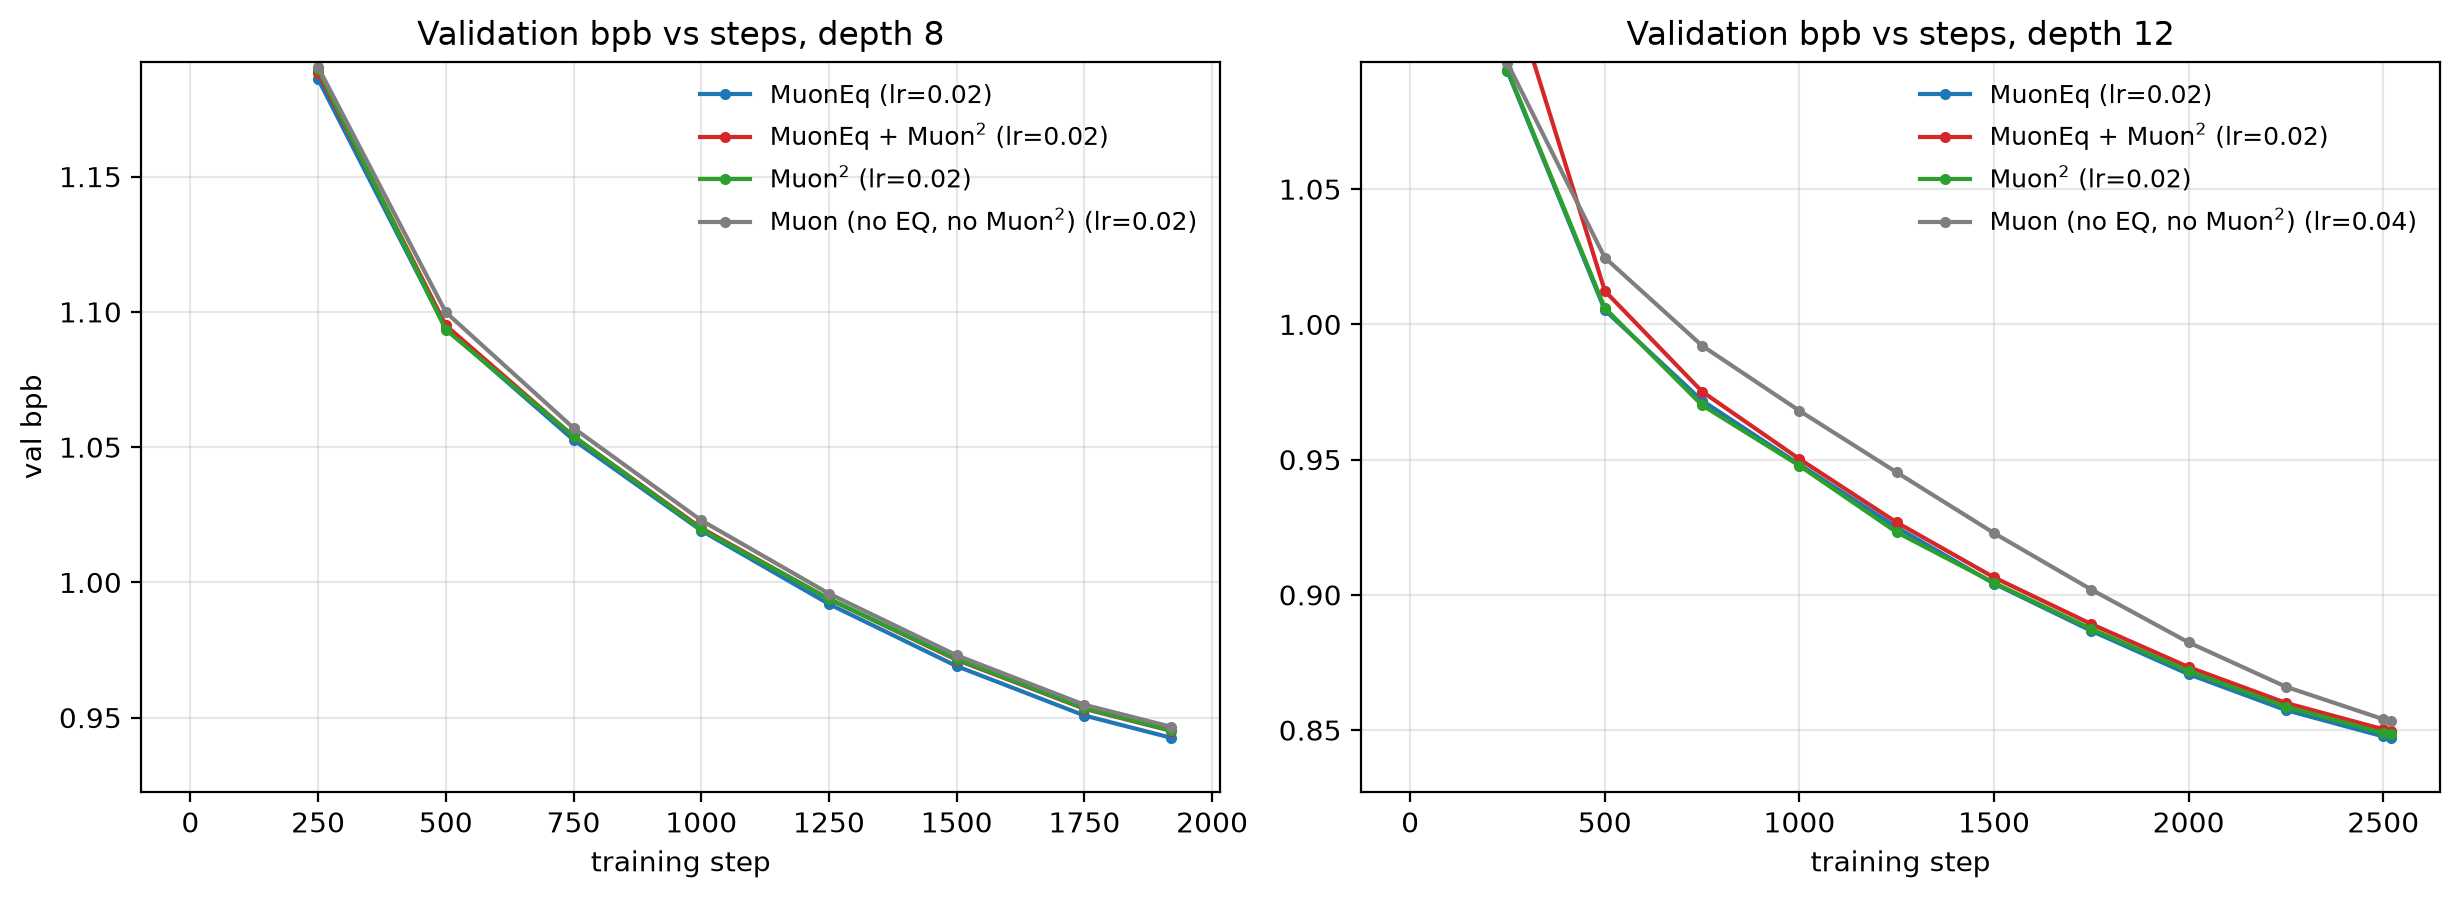
\includegraphics[width=\linewidth]{results/figures/plain_val_bpb_vs_steps.png}
    \caption{Validation bpb as a function of training step for each optimizer variant without post-orthogonalization extensions. Each subfigure corresponds to a different depth.}
    \label{fig:plain-val-vs-steps}
\end{figure}








\end{document}